%% Created by M.Sc. Nils Lutz
%%    For questions, comments, suggestions etc. send an email to:
%%    info@nilslutz.de
%%
%% Version: September 17, 2019
%%
%% Note: Has only been tested with pdflatex, not latex (dvi). Still, there is
%% theoretical support also for latex.
%%
\documentclass[enabledeprecatedfontcommands,12pt,bibtotoc]{scrartcl}

%% packages
\usepackage[T1]{fontenc}
\usepackage[utf8]{inputenc}       % Standard for Linux
\usepackage{lmodern}
%\usepackage[latin1]{inputenc}    % Standard for Windows
\usepackage{ngerman}              % For German language
\usepackage{fancyhdr}
\usepackage{geometry}
\usepackage{ifpdf}
\usepackage{setspace}             % For line spread
\usepackage[printonlyused, withpage, smaller]{acronym}
\usepackage[authoryear, round, sort]{natbib}
\usepackage{csquotes}
\renewcommand{\mkbegdispquote}[2]{\itshape}
\usepackage{enumitem}
\usepackage{tabularx}
\usepackage{booktabs}
\usepackage{lscape}
\usepackage[table,xcdraw]{xcolor}
\usepackage{color}
\usepackage{inconsolata}
\usepackage{float}
\usepackage{nicefrac}
\usepackage{listings} %For code in appendix
\usepackage{textcomp} % for upquote
\usepackage{blindtext}
\usepackage{float}
\usepackage{wrapfig}

\definecolor{pblue}{rgb}{0.13,0.13,1}
\definecolor{pgreen}{rgb}{0,0.5,0}
\definecolor{pred}{rgb}{0.9,0,0}
\definecolor{pgrey}{rgb}{0.46,0.45,0.48}

\usepackage{listings}
\lstset{language=Java,
  showspaces=false,
  showtabs=false,
  breaklines=true,
  showstringspaces=false,
  breakatwhitespace=true,
  belowskip=1ex,
  columns=fullflexible,
  commentstyle=\color{pgreen},
  keywordstyle=\color{pblue},
  stringstyle=\color{pred},
  framerule=0pt,
  numbers=left,
  tabsize=1,
   framexrightmargin=0em,
   framexleftmargin=0em,
  basicstyle=\ttfamily,
  moredelim=[il][\textcolor{pgrey}]{$$},
  moredelim=[is][\textcolor{pgrey}]{\%\%}{\%\%}
}



% For pdflatex
\ifpdf
  % One of these two:
  \usepackage[pdftex]{graphicx}
  %\usepackage[pdftex]{epsfig}

  \usepackage[pdftex]{hyperref}
% For latex (dvi)
\else
  % One of these two:
  \usepackage[dvips]{graphicx}
  %\usepackage[dvips]{epsfig}

  % make the command \href from hyperref available as a 'print only'
  \newcommand{\href}[2]{#2}
\fi

%% Picture options
\graphicspath{{pictures/}}         % Default path to pictures used
\DeclareGraphicsExtensions{.png}   % More extensions can be added

% Hyper ref coloring
\hypersetup{colorlinks, citecolor=black, linkcolor= black, urlcolor=black}

%% Pagestyle options
\pagestyle{fancy}
%\lhead{}
%\chead{}
%\rhead{}
%\lfoot{Daniel Süpke}
%\cfoot{}
%\rfoot{}
\renewcommand{\headrulewidth}{0.4pt}

\geometry{a4paper,left=3cm,right=3cm}
%\geometry{a4paper,left=3cm,right=2.5cm}   % Please use these settings for a PhD-thesis

%% Document start
\begin{document}

\pagenumbering{Roman}

% Insert titlepage
%% Title page

%\chead{}
%\rhead{}
%\lfoot{Daniel Süpke}
%\cfoot{}
%\rfoot{}
\begin{titlepage}

  \begin{centering}
  \begin{figure}[h!]
    \centering
    
\includegraphics[width=310pt]{Jade_Logo}
  \end{figure}

  %\vspace*{-0.8cm}

  % \begin{figure}[h!]
  %   \centering
  %   
\includegraphics[width=250pt]{Logo_Department}
  % \end{figure}

  \vspace*{0.4cm}

  \textsf{\Huge \textbf{Prüfungsleistung ED
  im Fach
  Datenbankgestützte Informationssysteme (DBIS)
  \\}}

  \vspace*{0.5cm}
  \textsf{\Huge Kassenbon-Data Warehouse, Umsätze und Analyse mit Aggregattabellen auf Wochenbasis
  \\}
  \vspace*{0.2 cm}
  \noindent Fachbereich: Management, Information, Technologie \\
Prof. Dr. Alfred Wulff

  \end{centering}

  \vspace*{1.5cm}

  \begin{center}
    \framebox{%
  \vbox{\begin{tabbing}
  Aufgabe: \hspace*{20mm} \= 13 \\
  Matrikelnummer:\> 6013868\\
  Name:\> Tokuc\\
  Vorname:\> Kübra\\
  Email:\> kuebra.tokuc@student.jade-hs.de\\
  Studiengang:\> Wirtschaftsinformatik \\
  Semester:\> WS2019/20 \\
  Abgabetermin:\> 16. Januar 2020
  \end{tabbing}}%
  }
  \end{center}

\end{titlepage}
%\thispagestyle{empty}
\newpage


% Insert table of contents
% Insert table of contents
\tableofcontents
\newpage

% Insert glossary, table of symbols, list of figures and list of tables

\newpage

\listoffigures
\addcontentsline{toc}{section}{Abbildungsverzeichnis}

\newpage


\pagenumbering{arabic}

%% Line spread
\onehalfspacing

% Insert introduction
\section{Aufgabenbeschreibung}
In diesem Abschnitt \citep[siehe auch][]{Gubbi2013} der Arbeit wird das Ziel formuliert, in einen größeren Zusammenhang eingeordnet und gegen andere Themen abgegrenzt. Die wichtigsten Begriffe des Themas müssen in der Einleitung präzise definiert werden; eine sorgfältige Formulierung ist hier besonders wichtig. Weiterhin können Hinweise zur verwendeten Untersuchungsmethodik gegeben werden. Durch die Darstellung des Gangs der Untersuchung kann auch die Zweckmäßigkeit der gewählten Gliederung hervorgehoben werden.  Nach Möglichkeit sollte dieses Kapitel nicht ‚Einleitung‘ heißen, sondern einen sinnvollen Titel mit Bezug zur Arbeit tragen.





% Insert body
\section{Pflichtenheft}
In diesem Kapitel werden die Kriterien für für die Erfüllung der Projektanforderungen kurz beschrieben.
% Insert here all subsection as file input
\subsection{Zielbestimmung}
\paragraph{Musskriterien}
\begin{enumerate}
  \item Richten Sie die Tabellen mit den bereitgestellten SQL-Skripten in Ihrer eigenen Datenbank
  des MS-SQL-Servers ein.
  \item Eines der gegebenen SQL-Skripte füllt die operationale Datenbank mit einem Grundbestand an Filialen und Produkten. Es existieren aber noch weitere PRODUKTE, die in der Datei \glqq PRODUKTE1.csv\grqq{} abgelegt sind. Erstellen Sie ein Java-Programm, das die zusätzlichen Daten in die operationale Datenbank klädt. In der CSV-Datei können fehlerhafte Daten enthalten sein. Führen Sie eine geeignete Fehlerbehandlung  und -protokollierung durch. Verwenden Sie das JDBC-API oder die Hibernate-Technologie (optional).
  \item In dem vorgegebenen SQL-Skript wird die operationale Datenbank auch mit einem Grundbestand an Kassenbons gefüllt. Erweitern Sie den Datenbestand um min. 40 Kassenbons mit durchschnittlich 3 Bonpositionen und 7 Handelsmarken sowie 10 Fachbereiche der Filiale 14. Der Dateiname mit den zugehörigen Anweisungen soll \glq 3-Insert-Student\grq{} lauten und im Projektordner \glq sql\grq{} abgelegt sein.
  \item Analysieren Sie das bereitgestellte STAR-Schema für ein Data-Warehouse, welches dem Händler die Umsatzanalyse und Auswertung von Verkäufen ermöglicht. Als Faktenattribute werden Kassenbondaten berücksichtigt. dAuswertungen sollen in Bezug auf Filiale, Abteilung, Produkt und Zeiträumen möglich sein. Die Faktendaten sollen tagesgenau gespeichert werden. Es sollen zusätzlich aggregierte Faktenwerte auf Wochenbasis verfügbar sein.
  \item Erstellen Sie geeignete ETL-SQL-Skripte (falls erforderlich DDL- unf DML-Anweisungen), um die Daten aus der operativen DB in das DW zu extrahieren.
  \item Entwickeln Sie eine DB-Prozedur namens DW-REPORT. Zu allen oder ausgewählten Merkmalen der vorhandenen Dimensionen sollen die in einem bestimmten Zeitraum erzielten Verkäufe (z.B. Umsätze, Verkaufsmengen) berechnet und angezeigt werden. Der gewünschte Zeitabschnitt sowie Parameter der Dimensionen sollen weitgehend variabel, d.h. vom Benutzer einstellbar sein. Die Prozedur wird zur Auswertung des DW eingesetzt. Sie liefert in der Konsole eines SQL-Editors die Ergebnisse der Auswertung. Der Report soll formatiert und übersichtlich gestaltet sein. Verwenden Sie keine Reporting-Dienste, sonder erstellen Sie den SQL-Report mittels SQL-Anweisungen aus den Vorlesungsunterlagen und der Online-Dokumentation des MS SQL-Servers. Ein Beispiel für einen Prozeduraufruf mit von Ihnen vorgschlagenen Parametern ist zwingend erforderlich.
\end{enumerate}

\paragraph{Kannkriterien}

\begin{itemize}
  \item Zusätzlich soll eine Visualisierung der Auswertungen mit der BI-Software QlikSense vorgenommen werden.
\end{itemize}



\subsection{Einsatz}
Überschriften werden in \LaTeX{} mit den Befehlen $\backslash$section\{\}, $\backslash$subsection\{\} und $\backslash$paragraph\{\} erezugt.

Jeder Überschrift sollte auf der tiefsten Gliederungsebene mindestens eine Seite Text folgen, davon mindestens zwei Zeilen auf derselben Seite. Es sollten nicht mehr als vier Gliederungsebenen verwendet werden.

Überschriften sollten in eine Zeile passen, damit Silbentrennungen vermieden werden können. Sollten Silbentrennungen in Ausnahmefällen erforderlich sein, ist sinngemäß zu trennen, also z.B. nicht Umweltin-formatik, sondern Umwelt-informatik.

\subsection{Umgebung}

\begin{enumerate}
  \item Software-Client
  \begin{itemize}
    \item Windows 10
    \item JAVA JDK und JDBC
  \end{itemize}
  \item Software-Server
  \begin{itemize}
    \item MS SQL-Server auf whv-fbmit3.hs-woe.de
  \end{itemize}
  \item Hardware \begin{itemize}
    \item Client: H401/H416a/W108 Pool Rechner
    \item Server: whv-fbmit3.hs-woe.de
  \end{itemize}
  \item Orgware: ERM
  \end{enumerate}





\subsection{Daten}
Es wird ein Grunddatenbestand bereitgestellt. Dieser ist gem. Zielbestimmungen zu erweitern. Wenn Sie für die zusätzlich erstellten Daten externe Quellen verwenden, so sind sie anzugeben. Änderungen der Datenstrukten sind zu dokumentieren.
\subsection{Performance}
keine spezifischen Anforderungen
\subsection{Qualitätsziele}
\begin{itemize}
  \item hohe Benutzerfreundlichkeit
  \item hohe Änderbarkeit
\end{itemize}
\subsection{Ablieferung der Ergebnisse}
Folgende Bestandteile sind anzugeben bzw. einzurichten:
\begin{enumerate}
  \item Alle DB-Schemata müssen auf der eigenen Datenbank auf dem SQL-Server whv.fbmit3.hs-woe.de eingerichtet werden. Alle Anwendungsdaten liegen in dieser DB und die Programme greifen auf die Daten zu. Multiuser-Fähigkeit sollte gewährleistet sein (durch die Angabe des Eigentümers der DB-Objekte in SQL-Statements). Die Prüfer melden sich am MS SQL-Server nicht mit ihren Login-Daten an. Deshalb müssen Sie sicherstellen, dass die Skripte durch andere DB-User aufgerufen werden können.
  \item Abgabe lauffähiger, getesteter und ausführbarer SQL-Prozeduren: \begin{itemize}
    \item Die Skripte und Prozeduren müssen ausführbar sein. Diese sind im Projektordner \textbf{sql} abzulegen.
    \item Ein Beispiel für den Prozeduraufruf muss erstellt werden.
    \item Das Java-Programm muss lauffähig und mittels bat-Datei realisiert sein
  \end{itemize}
  \item Folgende Unternlagen sollen in gedruckter Form vorgelegt werden: \begin{itemize}
    \item Pflichtenheft/Aufgabenstellung
    \item Lösungswegbeschreibungen für (1) ETL-Prozess, (2) DW-REPORT (inkl. SQL-Anweisungen, Skripte, Prozeduren, Views, Trigger etc.) sowie zusätlich erstellte Tabellen udn Formeln.
    \item extra ausgedruckt: Java-Quellcode und SQL-Skripte mit Kommentaren und Erläuterungen
    \item Benutzerhandbuch für Anwendung des DW-Report
  \end{itemize}
  \item Folgende Unternlagen sollen in elektronischer Form (CD/DVD) vorgelegt werden: \begin{itemize}
    \item Alle gedruckten Unternlagen
    \item Alle Java-Programme und selbst erstellen SQL-Skripte
  \end{itemize}
  \item Abgabe in einem heftbaren Ordner inklusive eines fest angebrachten, leicht abnehmbaren Datenträgers.
\end{enumerate}
\subsection{Selbstständige Erarbeitung der Ergebnisse}
Die Ergebnisse von jedem Prüfling müssen selbst erbracht werden. Wer versucht, das Ergebnis ihrer Prüfungsleistung durch Täuschung oder Benutzung nicht zugelassener Hilfsmitteln (Entwurfs- und Programmbestandteile anderer Studierender) zu beeinflussen, wird mit \textbf{nicht ausreichend} bewertet.
\subsection{Organisatorisches}
\begin{itemize}
  \item Abgabe am 16.01.2020 (09:00. W108). Jeder Studierende muss zur Abgabe der Dokumentation persönlich erscheinen und dem Prüfer die Ergebnisse vorstellen.
\end{itemize}



% Insert conclusion
\section{Umsetzung}
\textcolor{red}{Zum Schluss der Arbeit kann in dem letzten Teil eine thesenartige Zusammenfassung der Untersuchungsergebnisse gegeben werden. Andere Möglichkeiten sind hier auch der Ausblick auf weitere – noch ungelöste – Fragestellungen im Zusammenhang mit dem Thema.}

\subsection{Einrichtung der Datenbank}

\begin{figure}[ht!]
  \centering
  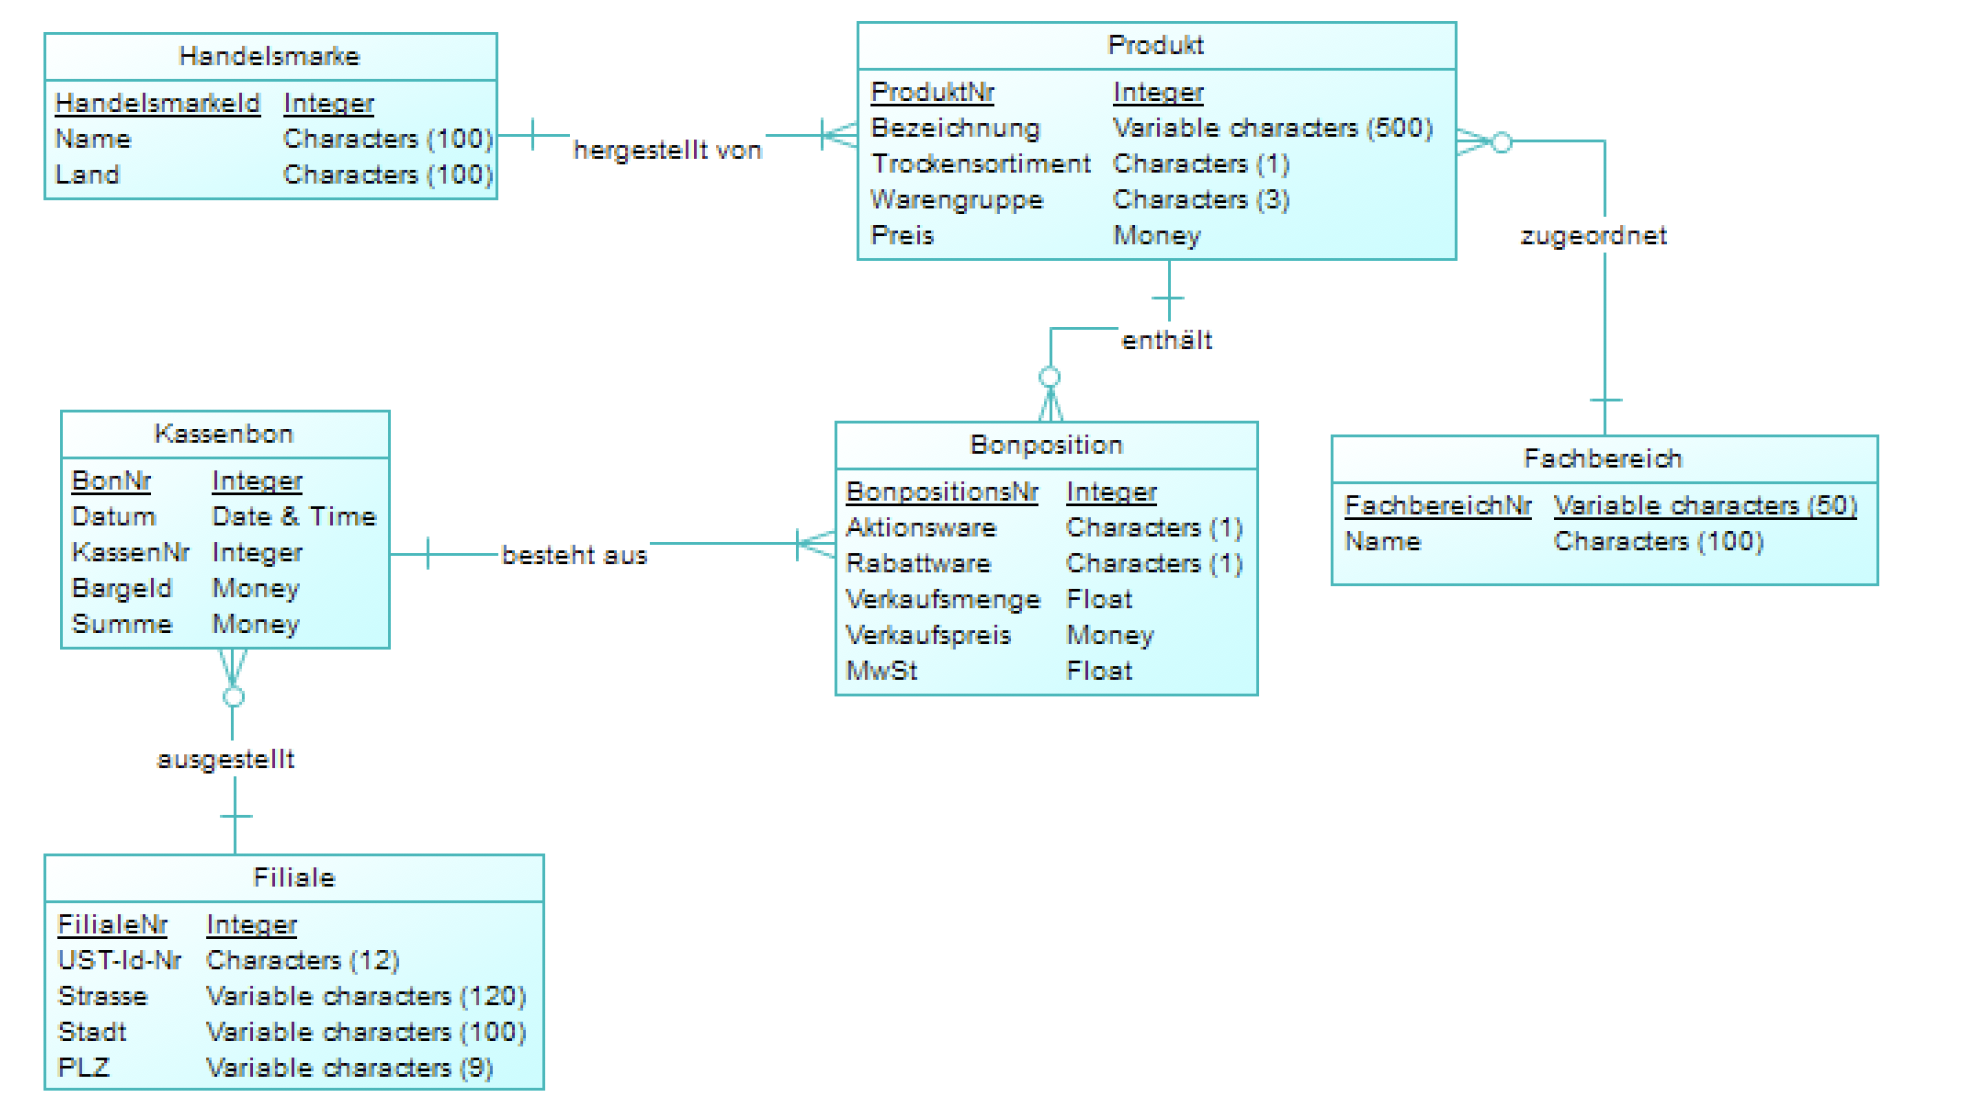
\includegraphics[width=1.2\linewidth]{pictures/db_basic.png}
  \caption[ER-Modell zur Auswertung von Kassenbons]{ER-Modell zur Auswertung von Kassenbons (Quelle: DBIS-Aufgaben)}
\end{figure}

\subsection{Java-Programm}


\begin{figure}[ht!]
  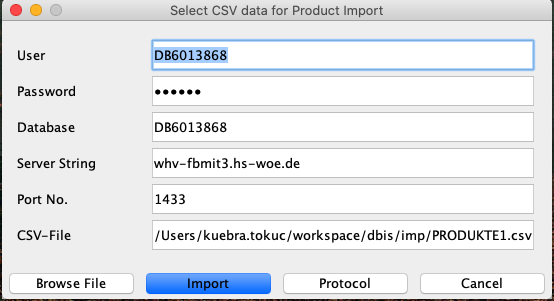
\includegraphics[width=1\linewidth]{window.png}
  \caption{Importfenster des Java-Programms}
\end{figure}


\textcolor{red}{\blindtext}

\subsection{Data Warehouse}

\subsubsection{Erweiterung des Datenbestandes}

\subsubsection{Aufbereitung des Datenbestandes}

\subsubsection{Analyse des Starschemas}

Nachdem der Datenbestand erweitert und korrekt aufbereitet worden ist, wird ein Starm-Schema für ein Data-Warehouse zur Umsatzanalyse und Auswertung von Verkaufsdaten nach einem vorliegenden Schema (s. Abbildung \ref{dw_concept}) erstellt. Das Star-Schema besteht aus Dimensionen- und Faktentabellen, welche die Struktur und den Inhalt einer multidimensionalen Datenmenge definieren \citep{Wulff2019}. Die Werte in der Faktentabelle werden durch die Primary Keys der Dimensionstabelle mit ihr in Abhängigkeit gebracht (s. Abbildung \ref{dw_phys}). Allerdings ergibt die Analyse des Datenmodells Inkosistenzen zwischen den verschiedenen Tabellen:

\begin{enumerate}
  \item Kein Fachbereich im Sternschema, stattdesen Abteilung
  \item Kassenbon\_Fakten AbteilungsNr FK int und DIM\_Abteilung AbteilungsNr PK int
  \item FilialeNr int der operativen DB und FilialeNr char(3) der DIM\_Filiale
  \item Warengruppe char(3) der operativen DB (ODB) und Warengruppe char(1) der DIM\_Produkt
  \item Bezeichnung des Produkts in ODB varchar(500) und in DIM\_Produkt varchar(100)
\end{enumerate}


\begin{figure}[ht!]
  \centering
  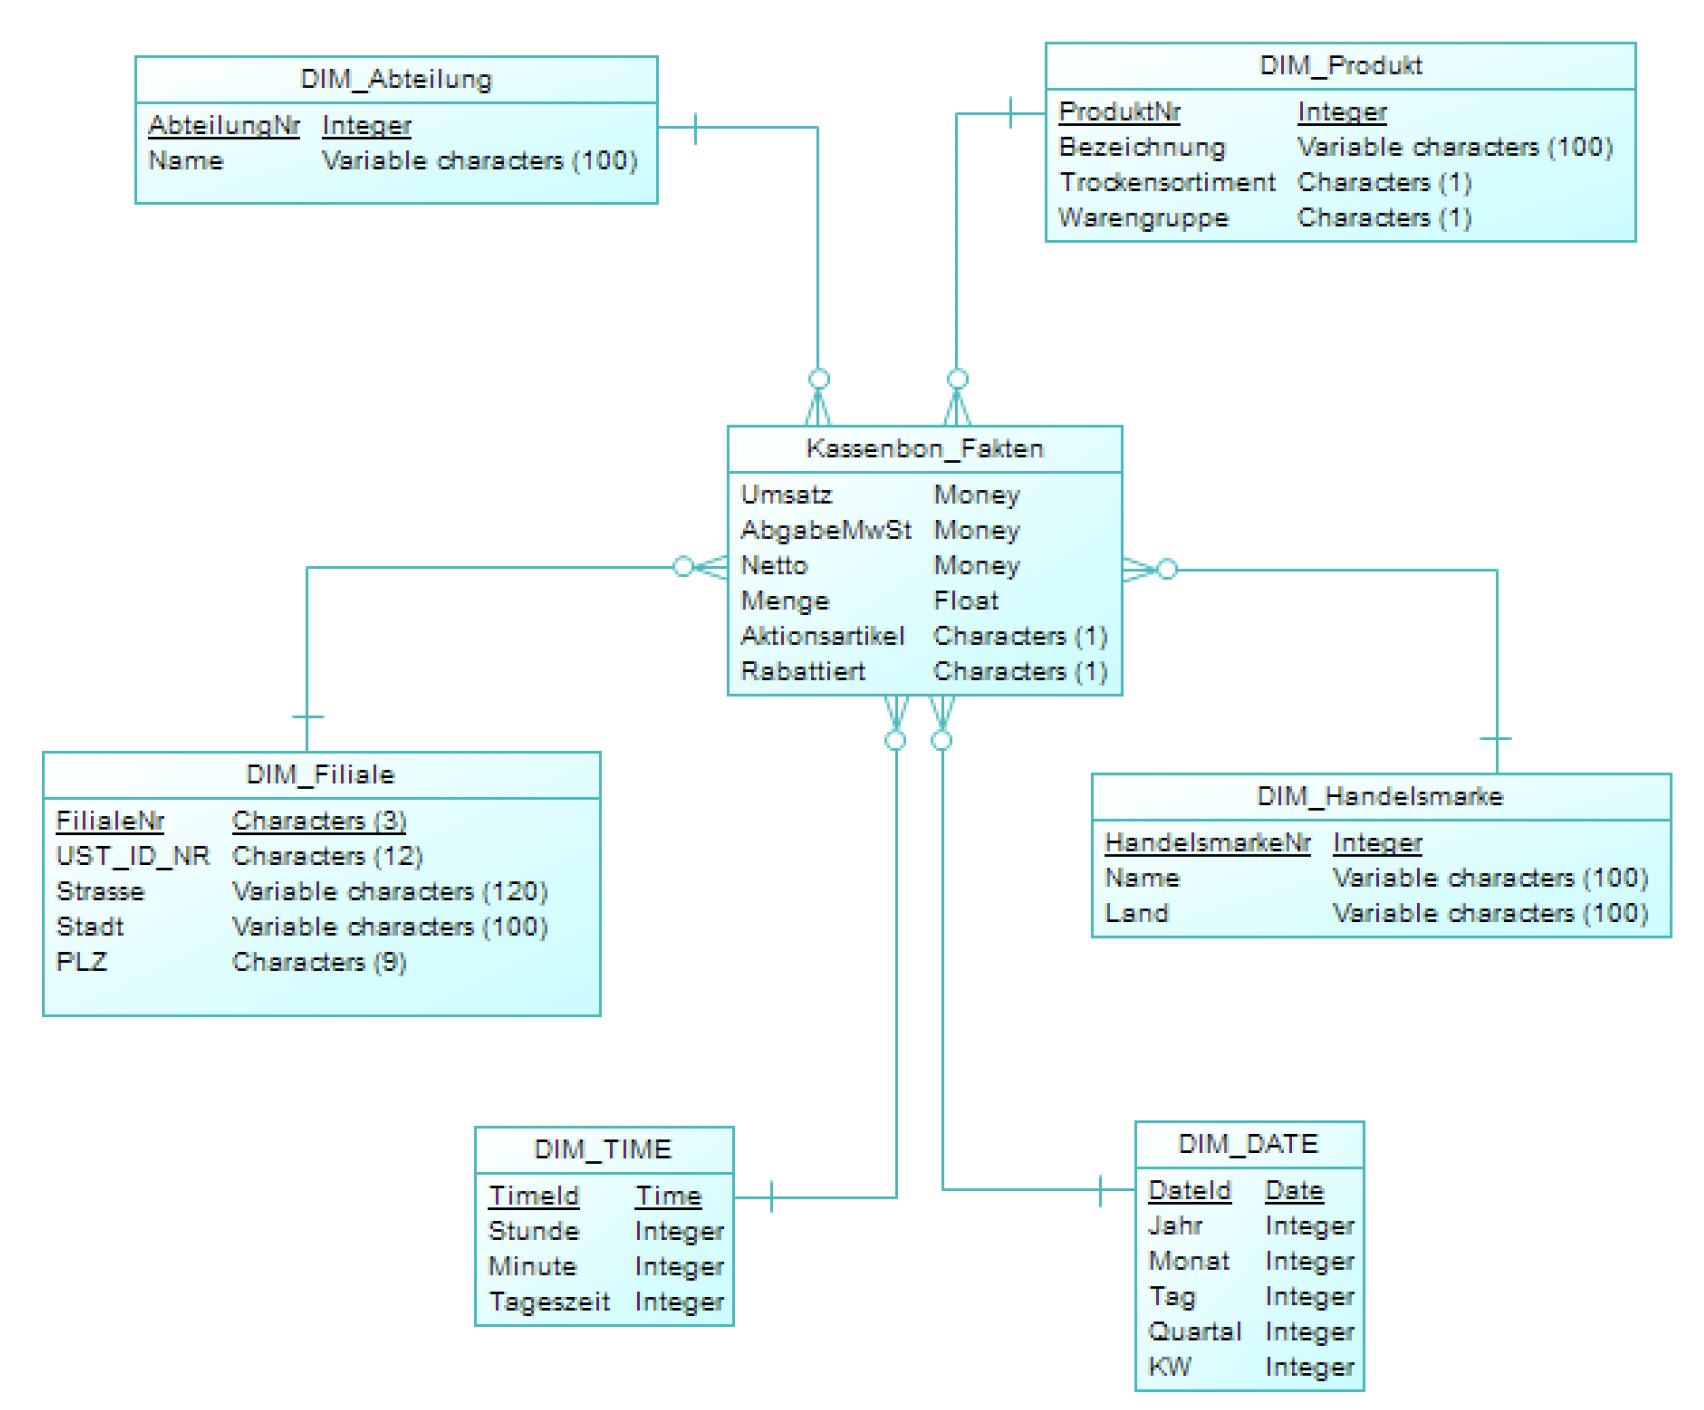
\includegraphics[width=1.1\linewidth]{pictures/dw_concept.png}
  \caption[Konzeptionelles Datenmodell des Data-Warehouses]{Konzeptionelles Datenmodell des Data-Warehouses (Quelle: DBIS-Aufgaben)}
  \label{dw_concept}
\end{figure}

\begin{figure}[ht!]
  \centering
  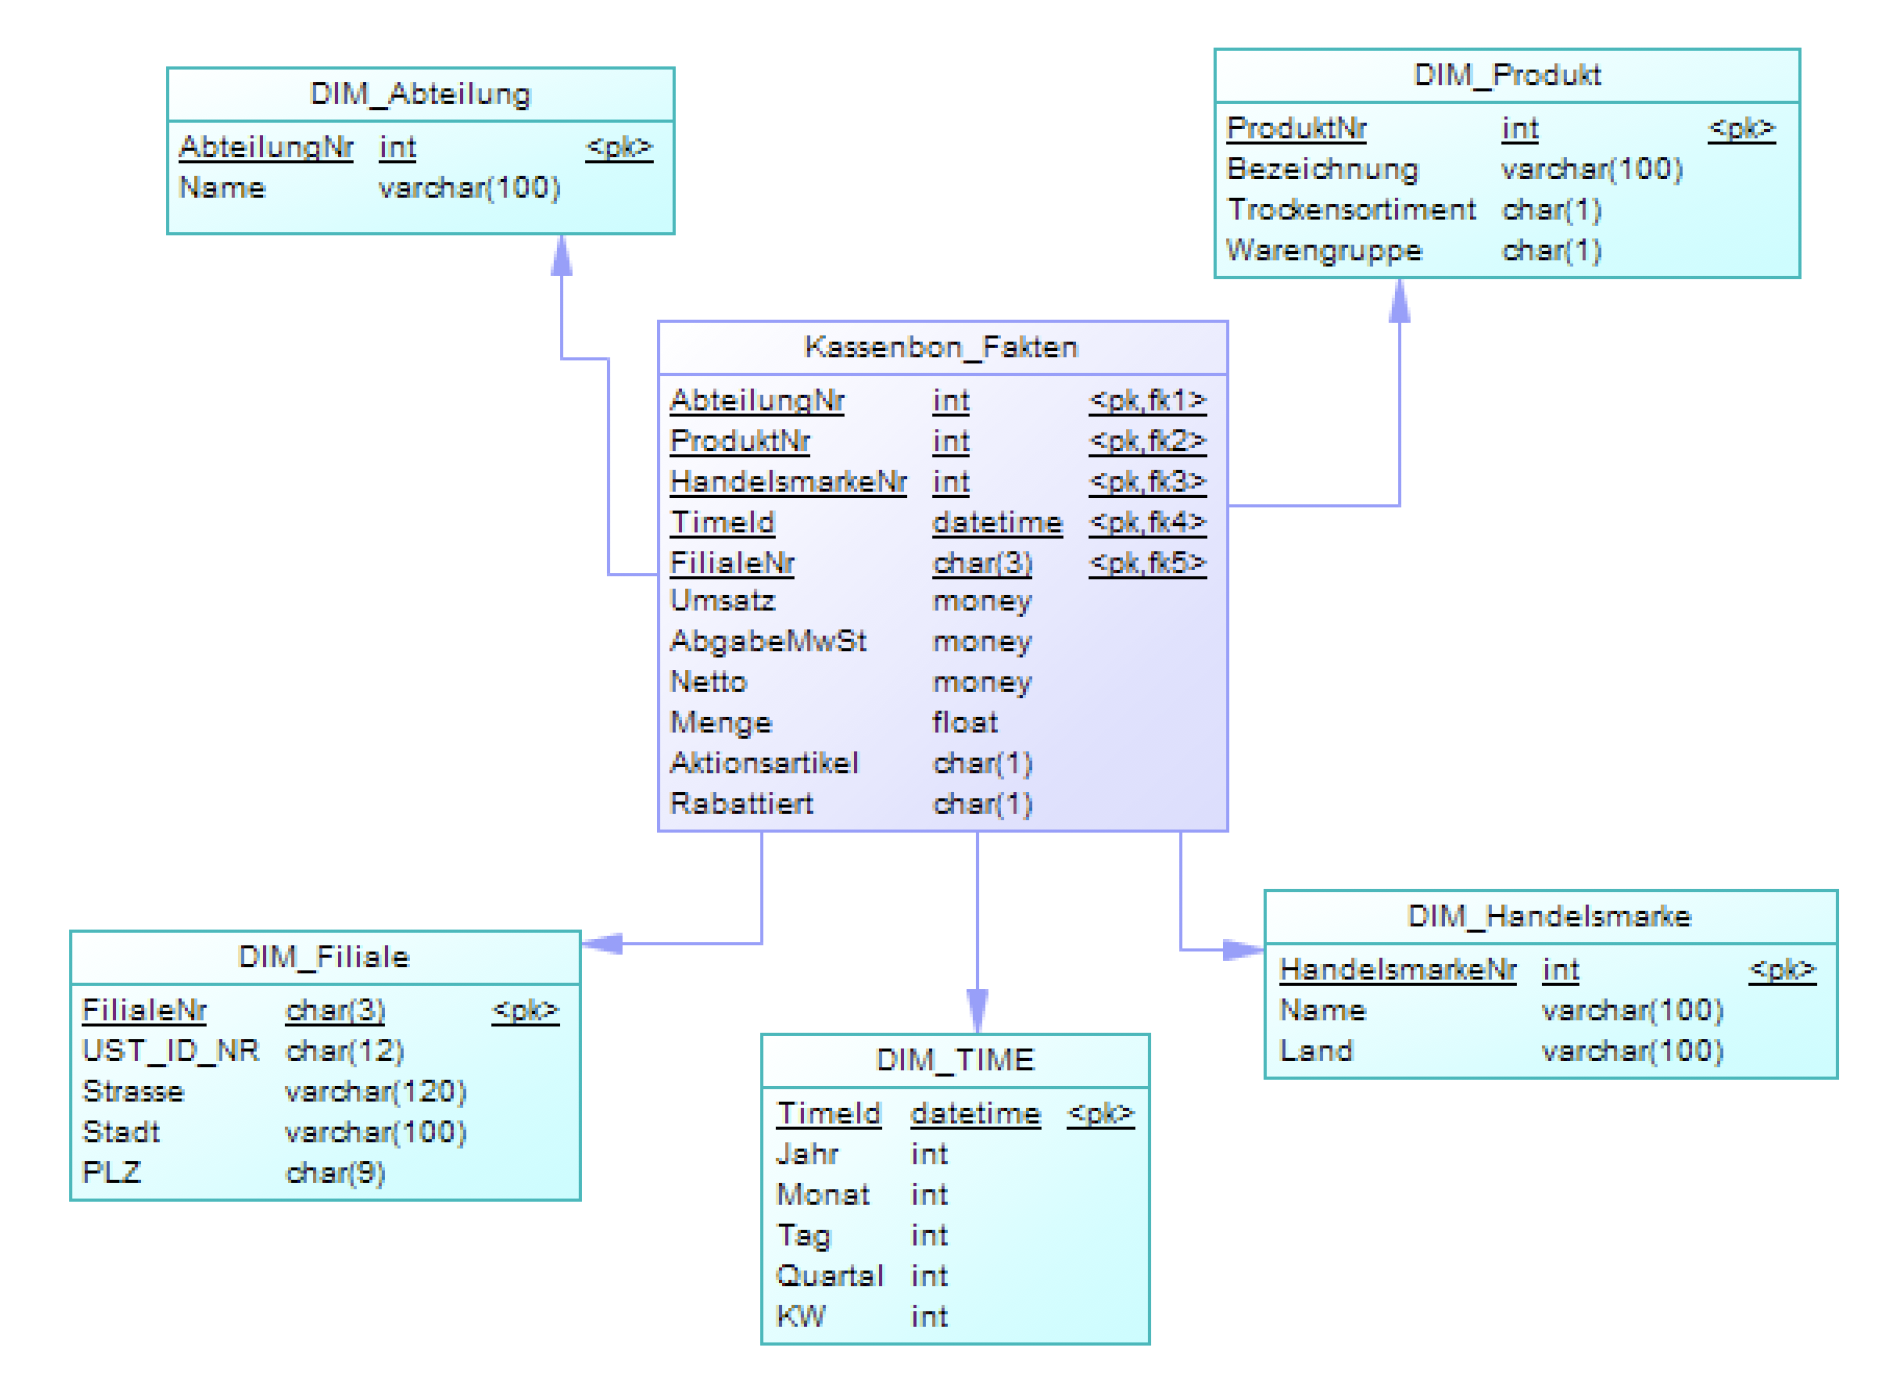
\includegraphics[width=1.1\linewidth]{pictures/DW_Physical_Data.png}
  \caption[Physikaliches Datenmodell des Data-Warehouses]{Physikaliches Datenmodell des Data-Warehouses (Quelle: DBIS-Aufgaben)}
  \label{dw_phys}
\end{figure}

\begin{figure}[ht!]
  \centering
  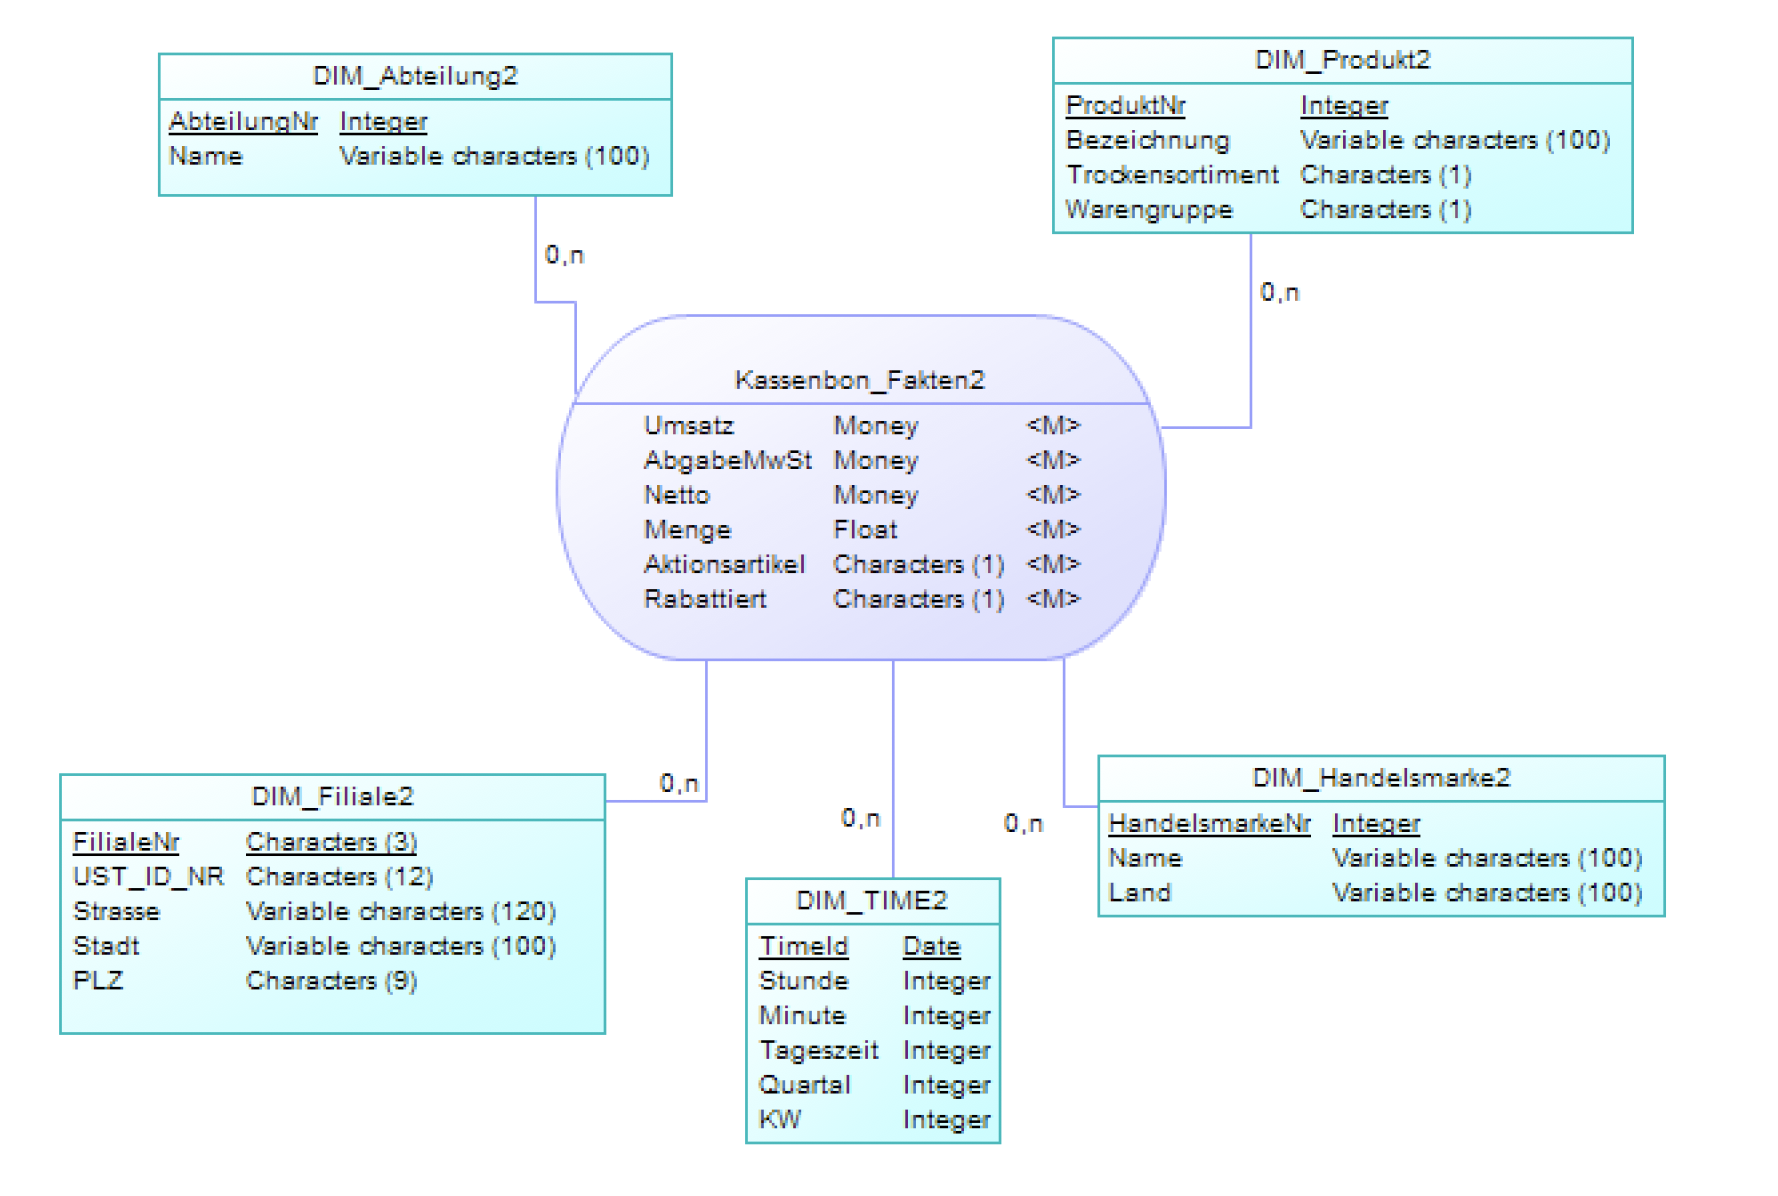
\includegraphics[width=1.1\linewidth]{pictures/dw_asso.png}
  \caption[Datenmodell des DW mit Assoziierung]{Datenmodell des DW mit Assoziierung (Quelle: DBIS-Aufgaben)}
  \label{dw_asso}
\end{figure}

\subsubsection{ETL-Prozess}

Mit dem ETL-Prozess (Extract, Transform, Load) werden die Daten aus der operativen Datenbank für die Auswertung und Analyse für das Laden in das Data-Warehouse aufbereitet.


\subsubsection{Aggregate auf Wochenbasis}

\begin{figure}[ht!]
  \centering
  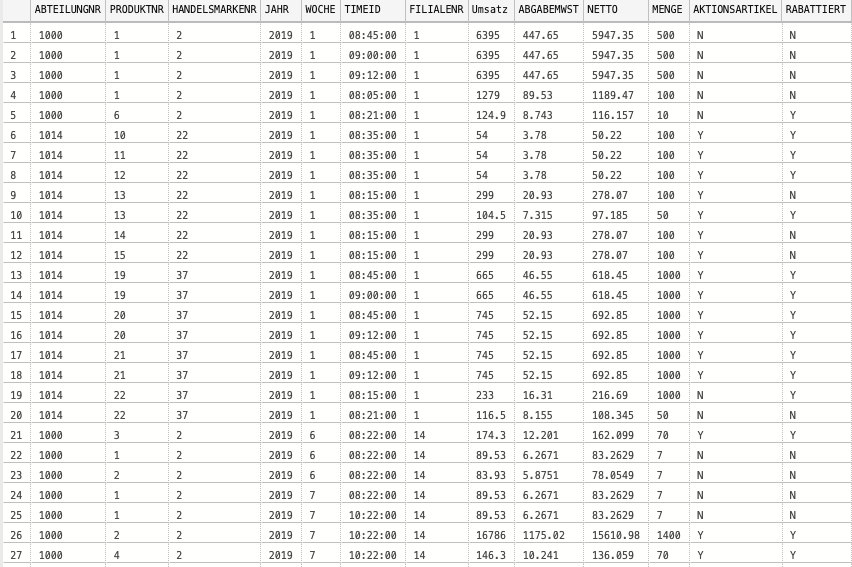
\includegraphics[width=1.1\linewidth]{pictures/fakten_woche.png}
  \caption{Aggregate auf Wochenbasis}
  \label{fakten_woche}
\end{figure}


\textcolor{red}{\blindtext}

\subsection{Prozedur für das Reporting}

\begin{figure}[ht!]
  \centering
  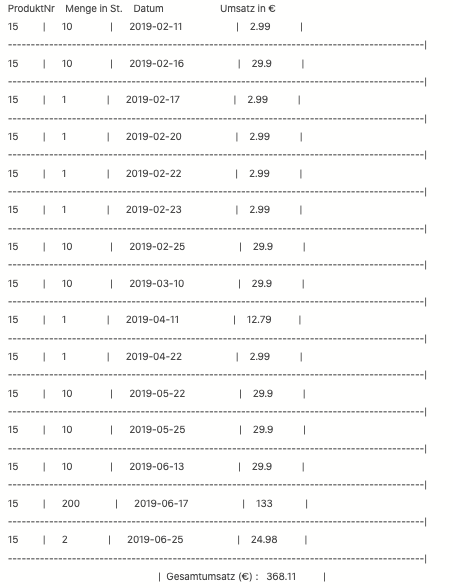
\includegraphics[width=1.1\linewidth]{pictures/report_sql.png}
  \caption{Reporting-Tabelle}
  \label{report_sql}
\end{figure}

\subsection{Reporting mit QlikSense}

\textcolor{red}{\blindtext}

\newpage



%\pagenumbering{Roman}
%\setcounter{page}{7}

% Insert bibliography
\newpage
\bibliographystyle{apalike}
\bibliography{thesis}

% Insert appendix
\newpage

\appendix

\section{Quelltext für das Java Programm}

\subsection{ImportWindow}

\begin{lstlisting}

  public class ImportWindow implements ActionListener{

	// Datenbankverbindung mit JDBC Data Source

	private DBConnection dbcon;
	private Connection con;
	private Statement statement;
	//LoginFenster
	public JFrame frmLoginWindow;
	//Logger
	private static final Logger LOG = Logger.getGlobal();

	//Labels for Connection Screen
	private JLabel userL;
	private JLabel passwordL;
	private JLabel databaseL;
	private JLabel serverL;
	private JLabel portL;
	private JLabel fileL;
	//Inputs in Connection Screen
	private JTextField userF;
	private JPasswordField passwordF;
	private JTextField databaseF;
	private JTextField fileF;
	private JTextField serverF;
	private JTextField portF;
	//Buttons for Screens
	private JButton btnImport;
	private JButton btnFile;
	private JButton btnCancel;
	private JButton btnProtocol;
	//Protocol
	private String protocol_content;

	//Constructor for starting Application Window
	public ImportWindow() {
		init();
	}

	public void init() {
		frmLoginWindow = new JFrame("Select CSV data for Product Import");
		frmLoginWindow.setBounds(100,100,550,300);
		frmLoginWindow.setDefaultCloseOperation(JFrame.EXIT_ON_CLOSE);
		frmLoginWindow.setLocationRelativeTo(null);
		frmLoginWindow.setResizable(false);

		userL = new JLabel("User");
		passwordL = new JLabel("Password");
		databaseL = new JLabel("Database");
		serverL = new JLabel("Server String");
		portL = new JLabel("Port No.");
		fileL = new JLabel("CSV-File");

		//Buttons
		btnImport = new JButton("Import");
		btnImport.addActionListener(this);
		btnFile = new JButton("Browse File");
		btnFile.addActionListener(this);
		btnCancel = new JButton("Cancel");
		btnCancel.addActionListener(this);
		btnProtocol = new JButton("Protocol");
		btnProtocol.addActionListener(this);

		// Input Fields

		userF = new JTextField();
		userF.setText("DB6013868");

		passwordF = new JPasswordField();
		passwordF.setText("3utbve");

		databaseF = new JTextField();
		databaseF.setText("DB6013868");

		serverF = new JTextField();
		serverF.setText("whv-fbmit3.hs-woe.de");

		portF= new JTextField();
		portF.setText("1433");

		fileF = new JTextField();
		fileF.setText(System.getProperty("user.dir")
				+ System.getProperty("file.separator") + "imp"
				+ System.getProperty("file.separator") + "PRODUKTE1.csv");

		//JPanel for Labels

		JPanel labelPane = new JPanel(new GridLayout(6, 1));
		labelPane.setBorder(BorderFactory.createEmptyBorder(15, 15, 15, 15));

		labelPane.add(userL);
		labelPane.add(passwordL);
		labelPane.add(databaseL);
		labelPane.add(serverL);
		labelPane.add(portL);
		labelPane.add(fileL);

		// JPanel for Inputs

		JPanel fieldPane = new JPanel(new GridLayout(6, 1));
		fieldPane.setBorder(BorderFactory.createEmptyBorder(15, 15, 15, 15));
		fieldPane.add(userF);
		fieldPane.add(passwordF);
		fieldPane.add(databaseF);
		fieldPane.add(serverF);
		fieldPane.add(portF);
		fieldPane.add(fileF);

		// JPanel for Buttons

		JPanel btnPane = new JPanel(new GridLayout(1,4));
		btnPane.add(btnFile);
		btnPane.add(btnImport);
		btnPane.add(btnProtocol);
		btnPane.add(btnCancel);

		//Container
		Container container = frmLoginWindow.getContentPane();
		container.setBackground(Color.lightGray);

		//Button Default
		frmLoginWindow.getRootPane().setDefaultButton(btnImport);

		//place panels
		container.add(labelPane, BorderLayout.CENTER);
		container.add(fieldPane, BorderLayout.LINE_END);
		container.add(btnPane, BorderLayout.SOUTH);

		frmLoginWindow.setVisible(true);
	}

	@Override
	public void actionPerformed(ActionEvent e) {

		if(e.getSource() == btnFile){
			final JFileChooser fc = new JFileChooser();
			int returnVal = fc.showOpenDialog(fc);

			if (returnVal == JFileChooser.APPROVE_OPTION) {
				File file = fc.getSelectedFile();
				//This is where a real application would open the file.
				fileF.setText(file.getAbsolutePath());
				LOG.info("File selected with success");
			}
			System.out.println("Button geklickt!");
		}
		else if(e.getSource() == btnCancel) {
			System.exit(0);
			System.out.println("Canceled");
			LOG.info("Canceled");
		}
		else if(e.getSource() == btnProtocol) {

			JTextArea outputArea = new JTextArea(20, 40);
			// Header and append
			String header = getHeader();
			String foot = getFoot();
			protocol_content = header + protocol_content + foot;
			outputArea.setText(protocol_content);
			outputArea.setEditable(false);
			JScrollPane scrollPane = new JScrollPane(outputArea);

			JOptionPane.showMessageDialog(new JFrame(), scrollPane, "Protokoll",
					JOptionPane.INFORMATION_MESSAGE);
		}
		// DB Import CSV
		else if(e.getSource() == btnImport) {

			LOG.info("Import clicked..");

			try {
				LOG.info("Connecting...");
				dbcon = new DBConnection(serverF.getText(),
						portF.getText(), databaseF.getText(),
						userF.getText(), new String(
								passwordF.getPassword()));
				con = dbcon.getConnection();

				// Testen der Verbindung

				boolean isOk = dbcon.testConnection();

				//Test if connection is established --> true!!
				System.out.println("Connection established"+ isOk);
				protocol_content+= "Connection established to" + " "+serverF.getText();


				if (!isOk) {
					JOptionPane.showMessageDialog(new JFrame(),
							"Die Anmeldung konnte nicht durchgefuhrt werden!"
									+ "\n\nBitte uberprufen Sie Ihre Angaben!",
									"Anmeldung fehlgeschlagen!", JOptionPane.ERROR_MESSAGE);
				} else {

					// Das Hauptfenster fur die Systemverwaltung wird geoffnet.
					ImportRoutine dbisImport = new ImportRoutine(con, fileF
							.getText());
					try {
						// Daten importieren
						protocol_content = dbisImport.startImport();

						if (dbisImport.isImportOk())
							JOptionPane.showMessageDialog(new JFrame(),
									"Datenimport wurde erfolgreich durchgefuhrt!", "Datenimport",
									JOptionPane.INFORMATION_MESSAGE);
						else
							JOptionPane.showMessageDialog(new JFrame(),
									"Datenimport wurde abgebrochen!",
									"Datenimport fehlgeschlagen!", JOptionPane.ERROR_MESSAGE);
					} catch (IOException e1) {
						JOptionPane
						.showMessageDialog(
								new JFrame(),
								"Die Datei konnte nicht gefunden oder nicht gelesen werden!"
										+ "\n\nBitte uberprufen Sie Pfad, Name und Rechte der Importdatei!",
										"Import fehlgeschlagen!", JOptionPane.ERROR_MESSAGE);
						e1.printStackTrace();
					}
					//****************!!!**************
					dbcon.freeConnection();
				}

			} catch (SQLException e1) {
				LOG.log(Level.SEVERE, "Fehler im Datensatz.", e1);
				JOptionPane.showMessageDialog(new JFrame(),
						"Keine Verbindung zur Datenbank!\n" +
								"Bitte Uberprufen Sie Ihre Angaben!",
								"Datenimport", JOptionPane.ERROR_MESSAGE);
			}
		}

	}
	private String getHeader() {
		return "**************************************\n" + "Start: "
				+ Date_Format.getDdMMyyyyHHMi(System.currentTimeMillis())
				+ " Uhr \n" + "Benutzer: " + userF.getText() + "\n" + "Database: "
				+ databaseF.getText() + "\n"
				+ "**************************************\n\n";
	}
	private String getFoot() {
		return "\n\n**************************************\n" + "End: "
				+ Date_Format.getDdMMyyyyHHMi(System.currentTimeMillis())
				+ " Uhr \n" + "**************************************\n\n";
	}


}

\end{lstlisting}

\subsection{DBConnection}

\begin{lstlisting}

  public class DBConnection {

	// Establish Connection via DataSource --> "mittlerweile bevorzugt"
	// i-net MERLIA.jar is JDBC 3.0 / 4.0 driver for MS SQL Server
	// Quelle 6. Dezember 2019: https://www.inetsoftware.de/products/jdbc-driver/ms-sql/features
	// Class.forName("com.inet.tds.TdsDriver") - MS-SQL-Server
	// This class is an implementation of a simple javax.sql.DataSource for the driver i-net ...
	// ... OPTA-xs and MERLIA-xs. For application servers you should use the PDataSource or DTCDataSource.
	// Quelle 6. Dezember TDSDataSource: https://www.inetsoftware.de/documentation/jdbc-driver/ms-sql/apispec/index.html?com/inet/tds/TdsDataSource.html
	// public TdsDataSource () Methods:
	// getConnection(username, password) throws java.sql.SQLException returns a Connection to database
	// setUrl(java.lang.String.jdbcUrl) and getUrl()
	// setServerName(String serverName)
	// getInstanceName()
	// setDatabaseName(String databaseName) etc ....
	// setPort(String port) --> cast from Textfield not necessary, if not set, default ist 1433
	// setUser and getUser as well as getPassword set Password both String


	private final String serverName;
	private final String port;
	private final String databaseName;
	private final String username;
	private final String password;
	private Connection con;
	private static final Logger log = Logger.getGlobal();

	// Constructor for DB-Connection-Object
	public DBConnection(String serverName, String port, String databaseName, String username, String password) {

		this.serverName = serverName;
		this.port = port;
		this.databaseName = databaseName;
		this.username = username;
		this.password = password;
	}

	public synchronized Connection getConnection() throws SQLException{

		// Connection with DataSource

		try {
			if (con == null || con.isClosed()) {
				DataSource ds = new TdsDataSource();
				((TdsDataSource) ds).setServerName(serverName);
				((TdsDataSource) ds).setPortNumber(Integer.parseInt(port));
				con = ds.getConnection(username, password);
				con.setCatalog(databaseName);
			}
		} catch (SQLException e) {
			log.log(Level.WARNING, "DB Connection failed.", e);
			JOptionPane.showMessageDialog(new JFrame(),
					" DB Connection failed!\n" +
							"Check your connection input",
							"CSV Import", JOptionPane.ERROR_MESSAGE);
		}
		return con;

	}
	public synchronized void freeConnection() {
		try {
			System.out.println("Active DB-Verbindung wird geschlossen... ");
			con.close();
			con = null;
		} catch (Exception e) {

		}
	}

	public synchronized boolean testConnection() {
		try {
			// Connection worked!
			log.info("Testing Connection in DBConnectionDataSource");
			if (getConnection() != null)
				return true;
		} catch (Exception e) {
			e.printStackTrace();
		}
		return false;

	}
	public String getSchemaname() {
	    return "dbo";
	  }


}


\end{lstlisting}


\subsection{FileLine}

\begin{lstlisting}
  public class FileLine {

	private int produktNummer;
	private String fachbereichNr;
	private int handelsmarkeId;
	private String bezeichnung;
	private String trockensortiment;
	private String warengruppe;
	private double preis;

	// Constructor for FileLine

	public FileLine(
			String fachbereichNr,
			int handelsmarkeId,
			String bezeichnung,
			String trockensortiment,
			String warengruppe,
			double preis
			) {
		this.fachbereichNr = fachbereichNr;
		this.handelsmarkeId = handelsmarkeId;
		this.bezeichnung = bezeichnung;
		this.trockensortiment = trockensortiment;
		this.warengruppe = warengruppe;
		this.preis = preis;
	}

	public int getProduktNummer() {
		return produktNummer;
	}

	public String getFachbereichNr() {
		return fachbereichNr;
	}

	public int getHandelsmarkeId() {
		return handelsmarkeId;
	}

	public String getBezeichnung() {
		return bezeichnung;
	}

	public String getTrockensortiment() {
		return trockensortiment;
	}

	public String getWarengruppe() {
		return warengruppe;
	}

	public double getPreis() {
		return preis;
	}


}
\end{lstlisting}

\subsection{FileLineParser}

\begin{lstlisting}

  public class FileLineParser {

	private static final int SPALTENANZAHL = 4;

	// Erzeugt aus der ubergebenen Zeile ein Object

	protected static FileLine getExpFileLine(String line)
			throws NoSuchElementException, SQLException {

		String	bezeichnung = getValue(line, 1).trim();
		String	trockensortiment = getValue(line, 2).trim();
		String	warengruppe = getValue(line, 3).trim();
		String	preis = getValue(line, 4).trim();
		String 	fb_id;

		//Versuch: Handelsmarke und Fachbereich integrieren
		//Hardcoded Idee fur Fachbereich: Methode getFachbereich wie getWarengruppe
		//--> Fachbereichsnummer ist der Foreign Key

		// Gewuerrze sind nicht als Fachbereich vorhanden

		//Schwieriger: Handelsmarke -> Bezeichnung nochmal Tokenizen (1. Stelle oder mit Regex wegen Dr Oetker und Kellogs)
		//Muss auch ein insert fur Handelsmarke geben, wenn nicht vorhanden
		// Neue Handelsmarken: Weber, Kellog's, Nestle, Basic, Schaer. Nick



		if(bezeichnung.length() >500) {
			bezeichnung.substring(0, 500);
		}
		if(trockensortiment.length() >1) {
			trockensortiment.substring(0, 1);
		}



		warengruppe = FileLineParser.getWarengruppe(warengruppe);
		fb_id = FileLineParser.getFachbereichsNummer(warengruppe);

		if(warengruppe.length() >3) {
			warengruppe.substring(0,3);
		}
		FileLine fileLineObj = null;
		try {

			fileLineObj = new FileLine(fb_id, 9,bezeichnung,trockensortiment,warengruppe, Float.parseFloat(preis));
		} catch (Exception e) {
			System.out
					.println("Parsefehler: Bitte uberprufen Sie das Format in dieser Zeile:"
							+ line);
			throw new NoSuchElementException();
		}
		return fileLineObj;
	}

	/**
	 * Liefert einen Wert, fur den entsprechenden Index
	 */

	private static String getValue(String line, int keyIndex)
			throws NoSuchElementException {
		String value = null;
		boolean isDub = false;

		StringTokenizer lineValues = new StringTokenizer(line, ";");
		int tokens = lineValues.countTokens();

		// Uberprufung der Spaltenanzahl
		if (tokens < SPALTENANZAHL) {
			// Falls mehr Tokens in Zeile als notwendige Spaltenzahl, Throw NoSuchElementException
			System.out.println("Falsches Format von Testdaten!"
					+ "Zu wenige Parameter gefunden: "
					+ tokens + " von " + SPALTENANZAHL + "Spalten.");
			throw new NoSuchElementException("Falsches Format der Daten!\n");
		} else if (tokens > SPALTENANZAHL) {
			System.out.println("Falsches Format von Testdaten!"
					+ " Zu viele Parameter gefunden: " + tokens + " von "
					+ SPALTENANZAHL + " Spalten.");
			throw new NoSuchElementException("Falsches Format der Daten!\n");
		}

		for (int i = 0; i < keyIndex; i++) {
			value = lineValues.nextToken();
		}

		// Checkt, ob der Wert redundante Werte hat

		isDub = isDub(value);
		if(isDub == true) {
			System.out.println("Falsches Format von Testdaten!"
					+ "Redundante Daten");
			throw new NoSuchElementException("Falsches Format der Daten!\n");
		}

		return value;
	}

	// Ubergabe der Warengruppennummer

	public static String getWarengruppe(String s_warengruppe) {

		if (s_warengruppe == null)
			return null;

		String warengruppe_id = null;

		if (s_warengruppe.equalsIgnoreCase("Milch"))
			warengruppe_id = "002";
		else if (s_warengruppe.equalsIgnoreCase("Musli & Cerealien"))
			warengruppe_id = "003";
		else if (s_warengruppe.equalsIgnoreCase("Saucen"))
			warengruppe_id = "004";
		else if (s_warengruppe.equalsIgnoreCase("Gewurze"))
			warengruppe_id = "005";
		else
			warengruppe_id = "006";

		return warengruppe_id;
	}

	// Ubergabe der Fachbereichsnummer
	// wird auch Fachbereich fuer Gewurze erstellen

	public static String getFachbereichsNummer(String warengruppe_id) throws SQLException {

		if (warengruppe_id==null) {
			return null;
		}
		String fb_id= null;
		if (warengruppe_id=="002") {
			fb_id= "1014";
		}else if(warengruppe_id == "003") {
			fb_id= "1023";
		}else if(warengruppe_id == "004") {
			fb_id= "1015";
		}else if(warengruppe_id == "005") {
			ImportRoutine.createNewFB("Gewurze", "1039");
			fb_id="1039";
		}

		return fb_id;
	}

	// Methode zum Prufen von Redundanten Eintragen

	public static boolean isDub(String bezeichnung) {

		String[] words = bezeichnung.split("[\\s+]");

		Map<String, Integer> occurrences = new HashMap<String, Integer>();

		boolean isdub =false;
		Integer oldCount=0;
		for ( String word : words ) {
			oldCount = occurrences.get(word);
			if ( oldCount == null ) {
				oldCount = 0;
			}
			occurrences.put(word, oldCount + 1);
			if(oldCount>2) isdub = true;
			System.out.println("oldcount : "+ oldCount+ "word"+ word + "isdub" + isdub);
		}
		System.out.println("IS DUB? :"+ isdub);
		return isdub;
	}

}

\end{lstlisting}

\subsection{ImportRoutine}

\begin{lstlisting}

  public class ImportRoutine {

    //Schnittstelle zum Importieren von Daten

      protected BufferedReader in;
      protected final int DOPPELTER_PRIMARY_KEY_FEHLER = 2601;
      protected final int DOPPELTER_UNIQUE_SCHLUSSEL_FEHLER = 2627;
      protected String fileIn;
      protected static Connection con;
      private boolean istImportOk = true;

      public ImportRoutine(Connection con, String fileIn) {
        this.con = con;
        this.fileIn = fileIn;
      }

      /**
       * Liest Datei aus und speichert sie in die Datenbank.
       */
      public String startImport() throws IOException {
        String protocol = "";
        if (con == null) {
          System.out
              .println("Datenbankverbindung muss initialisiert werden!");
        }
        try {
          try {
            // Buffer fur Zeilen
          in = new BufferedReader(new FileReader(fileIn));
          }
          catch (Exception e) {e.printStackTrace();}

          String line = null;
          int lineCounter = 0;
          int objCounter = 0;

          protocol += "Datenimport wird gestartet...\n\n";

          // Abbruch des Exports bei falschen Zeilen

          try {
            line = in.readLine();
          }
          catch (IOException e1) {
            // TODO Auto-generated catch block
            e1.printStackTrace();
          }

          while (line != null && istImportOk) {
            lineCounter++;

            // Konmentare ausschliessen
            if (!line.trim().equals("") && !line.substring(0, 1).equals("#")) {
              try {
                // Zeile ueberspringen
                objCounter++;
                FileLine fileLine = FileLineParser.getExpFileLine(line);
                DBImport.insert(fileLine, con);

              } catch (SQLException e) {

                // Fehler ignorieren, wenn Zeile existiert

                if (e.getErrorCode() != DOPPELTER_PRIMARY_KEY_FEHLER
                    && e.getErrorCode() != DOPPELTER_UNIQUE_SCHLUSSEL_FEHLER) {
                  // Der Import soll weiter laufen, wenn der Datensatz
                  // existiert.
                  // istImportOk = false;
                  e.printStackTrace();
                  protocol += "SQL-Exception in der Zeile: "
                      + lineCounter + "\n";
                  protocol += line + "\n\n";
                  JOptionPane
                      .showMessageDialog(
                          new JFrame(),
                          "Daten aus der Zeile "
                              + lineCounter
                              + " verursachten beim Ausfuhren der SQL-Anweisung Fehler."
                              + "\nBitte uberprufen Sie die SQL-Anweisung oder zu importierenden Daten!",
                          "Datenimport",
                          JOptionPane.ERROR_MESSAGE);
                } else {
                  protocol += "Datensatz in der Zeile " + lineCounter + " ist bereits vorhanden:\n";
                  protocol += line + "\n\n";
                }
              } catch (ClassNotFoundException e) {
                // istImportOk = false;
                JOptionPane
                    .showMessageDialog(
                        new JFrame(),
                        "Keine Verbindung zur Datenbank!"
                            + "\nBitte uberprufen Sie Ihre Angaben!",
                        "Datenimport",
                        JOptionPane.ERROR_MESSAGE);
                e.printStackTrace();
                protocol += "Keine Verbindung zur Datenbank!\n\n";
                break;
              } catch (NoSuchElementException e) {
                protocol += "Parse-Exception in der Zeile: "
                    + lineCounter + "\n";
                protocol += line + "\n\n";
                JOptionPane
                    .showMessageDialog(
                        new JFrame(),
                        "Daten aus der Zeile "
                            + lineCounter
                            + " konnten nicht importiert werden."
                            + "\nBitte uberprufen Sie die zu importierenden Daten!",
                        "Datenimport",
                        JOptionPane.ERROR_MESSAGE);
                e.printStackTrace();
                // break;
              }
            }
            try {
              line = in.readLine();
            } catch (IOException e) {
              // TODO Auto-generated catch block
              e.printStackTrace();
            }
          }
          protocol += "Anzahl der verarbeiteten Datensatze: " + objCounter + "\n\n";
          protocol += "Datenimport ist abgeschlossen.\n\n";
        } finally {
          if (in != null)
            try {
              in.close();
            } catch (IOException e) {
              // TODO Auto-generated catch block
              e.printStackTrace();
            }
        }
        return protocol;
      }

      // Neuer Fachbereich fur Gewurze erstellen, bevor der Import vollzogen wird

      public static void createNewFB(String name, String fb_nr) throws SQLException {

        DBImport.insertFB(name, fb_nr, con);

      }

      /**
       * Liefert true, wenn der Import ohne Fehler durchgefuhrt wurde.
       */
      public boolean isImportOk() {
        return istImportOk;
      }

  }


\end{lstlisting}


\subsection{DBImport}

\begin{lstlisting}

  // Klasse zum Importieren der CSV-Zeilen in die Datenbank

public class DBImport{

	/**
	 * Speichert Daten der ubergebenen Zeile in der Datenbank.
	 *
	 * @throws ClassNotFoundException
	 */

	 // Schreiben der Daten in die Datenbank

	public static int insert(FileLine fileLine, Connection con)
			throws SQLException, ClassNotFoundException, NoSuchElementException {
		PreparedStatement stmnt = null;


		int ergebnisZeilen = 0;


		if (fileLine.getFachbereichNr() != null) {
			stmnt = con
					.prepareStatement("INSERT INTO "
							+ "dbo.PRODUKT"
							+"(fachbereichNr,handelsmarkeID,bezeichnung,trockensortiment,warengruppe,preis)"
							+"VALUES (?,?,?,?,?,?)");


			// Werte setzen:
			stmnt.setString(1, fileLine.getFachbereichNr());
			stmnt.setInt(2,fileLine.getHandelsmarkeId());
			stmnt.setString(3, fileLine.getBezeichnung());
			stmnt.setString(4, fileLine.getTrockensortiment());
			stmnt.setString(5,fileLine.getWarengruppe());
			stmnt.setDouble(6,fileLine.getPreis());

			System.out.println(fileLine.toString());
			// Insert Ausfuhren
			ergebnisZeilen = stmnt.executeUpdate();

			// Transaktion beenden:
			con.commit();
			con.setAutoCommit(true);
		} else
			throw new NoSuchElementException();

		if (stmnt != null)
			try {
				stmnt.close();
			} catch (Exception ex) {
			}
		stmnt = null;



		return ergebnisZeilen;
	}

	// Method for creating new Fachbereich

	@SuppressWarnings("null")
	public static void insertFB (String name, String fb_nr, Connection con) throws SQLException{


		int ergebnisZeilen = 0;


		String query = "INSERT INTO dbo.FACHBEREICH"
					+ "(FACHBEREICHNR, NAME)"
					+"VALUES (?,?)" ;

		PreparedStatement statement = con.prepareStatement(query);

		// Fachbereich will be created with number and name

		statement.setString(1,fb_nr);
		statement.setString(2,name);
		ergebnisZeilen = statement.executeUpdate();

		con.commit();
		con.setAutoCommit(true);
		if (statement != null)
			try {
				System.out.println("Inserting FB");
				statement.close();
			} catch (Exception ex) {
			}
		statement = null;


	}
}

\end{lstlisting}

\subsection{DateFormat}

\begin{lstlisting}


public class Date_Format {

	/**
	   * Liefert das Datum im Format "dd.MM.yyyy" zuruck.
	   * @param time long
	   * @return String
	   */
	  public static String getDdMMyyyyHHMi(long time) {
	    java.util.Date d = new java.util.Date(time);
	    TimeZone z = TimeZone.getDefault();

	    Calendar c = Calendar.getInstance(z, Locale.GERMANY);
	    SimpleDateFormat sd = new SimpleDateFormat("dd.MM.yyyy HH:mm:ss");
	    sd.setCalendar(c);
	    return sd.format(d);
	  }

	  /**
	   * Wandelt Datum als String in einen Longwert.
	   */
	  public static long getDdMMyyyy(String sDate) throws ParseException {
	    if ( (sDate == null) || sDate.trim().equals("")) {
	      return 0;
	    }
	    SimpleDateFormat dateFormat = new SimpleDateFormat("dd.MM.yyyy");
	    // Pruft, dass es sich tatsachlich um die richtigen Datumsangaben handelt.
	    dateFormat.setLenient(false);
	    GregorianCalendar date = new GregorianCalendar();
	    date.setTime(dateFormat.parse(sDate));
	    return date.getTime().getTime();
	  }

	  /**
	   * Wandelt Datum als String in ein GregorianCalendar-Objekttyp.
	   */
	  public static GregorianCalendar getDayAsGregorianCalendar(String sDate) throws ParseException {
	    if ( (sDate == null) || sDate.trim().equals("")) {
	      return null;
	    }
	    SimpleDateFormat dateFormat = new SimpleDateFormat("dd.MM.yyyy");
	    // Pruft, dass es sich tatsachlich um die richtigen Datumsangaben handelt.
	    dateFormat.setLenient(false);
	    GregorianCalendar date = new GregorianCalendar();
	    date.setTime(dateFormat.parse(sDate));
	    return date;
	  }

	  /**
	   * Wandel Date-Objekt in einen String im Format 'YYYY-MM-dd'
	   */
	    public static String getYyyyMMdd(java.sql.Date time) {
	      TimeZone z = TimeZone.getDefault();

	      Calendar c = Calendar.getInstance(z, Locale.GERMANY);
	      SimpleDateFormat sd = new SimpleDateFormat("yyyy-MM-dd");
	      sd.setCalendar(c);
	      return sd.format(time);
	    }

	    /**
	     * Wandel Long-Objekt in einen Date-Objekt
	     */
	    public static java.sql.Date getDate(long time) {
	      return new java.sql.Date(time);
	    }
}


\end{lstlisting}


\section{Quelltext für SQL-Skripte}

\subsection{3-Insert-Student}

\begin{lstlisting}

  -- ******************** Kassenbonerstellung *************************** --

insert into KASSENBON (FILIALENR, DATUM, KASSENNR, BARGELD, SUMME)
VALUES

(14, CONVERT([datetime], '2019-02-10 08:22:00.000', 20), 1, 400.00, 400.00),
(14, CONVERT([datetime], '2019-02-11 10:22:00.000', 20), 1, 33.00, 33.00),
(14, CONVERT([datetime], '2019-02-16 08:22:00.000', 20), 1, 12.00, 12.00),
(14, CONVERT([datetime], '2019-02-17 10:22:00.000', 20), 1, 123.00, 150.00),
(14, CONVERT([datetime], '2019-02-20 11:29:00.000', 20), 1, 134.00, 200.00),
(14, CONVERT([datetime], '2019-02-22 13:22:00.000', 20), 1, 22.00, 100.00),
(14, CONVERT([datetime], '2019-02-23 14:25:00.000', 20), 1, 43.00, 50.00),
(14, CONVERT([datetime], '2019-02-25 08:30:00.000', 20), 1, 40.00, 100.00),
(14, CONVERT([datetime], '2019-03-10 12:29:00.000', 20), 1, 100.00, 100.00),
(14, CONVERT([datetime], '2019-04-22 14:20:00.000', 20), 1, 223.00, 230.00),
(14, CONVERT([datetime], '2019-04-11 13:20:00.000', 20), 1, 433.00, 450.00),
(14, CONVERT([datetime], '2019-05-22 15:20:00.000', 20), 1, 333.00, 335.00),
(14, CONVERT([datetime], '2019-05-23 14:40:00.000', 20), 1, 555.00, 555.00),
(14, CONVERT([datetime], '2019-05-24 16:22:00.000', 20), 1, 244.00, 250.00),
(14, CONVERT([datetime], '2019-05-25 15:30:00.000', 20), 1, 260.00, 260.00),
(14, CONVERT([datetime], '2019-05-25 16:23:00.000', 20), 1, 50.00, 50.00),
(14, CONVERT([datetime], '2019-05-25 16:45:00.000', 20), 1, 78.44, 100.00),
(14, CONVERT([datetime], '2019-05-25 17:44:00.000', 20), 1, 444.00, 450.00),
(14, CONVERT([datetime], '2019-05-26 17:55:00.000', 20), 1, 50.00, 50.00),
(14, CONVERT([datetime], '2019-05-27 12:42:00.000', 20), 1, 33.50, 35.00),
(14, CONVERT([datetime], '2019-05-28 17:50:00.000', 20), 1, 447.00, 450.00),
(14, CONVERT([datetime], '2019-06-02 12:44:00.000', 20), 1, 1000.00, 1000.00),
(14, CONVERT([datetime], '2019-06-12 10:44:00.000', 20), 1, 23.00, 34.00),
(14, CONVERT([datetime], '2019-06-12 12:44:00.000', 20), 1, 25.00, 37.00),
(14, CONVERT([datetime], '2019-06-13 10:44:00.000', 20), 1, 399.00, 400.00),
(14, CONVERT([datetime], '2019-06-14 12:44:00.000', 20), 1, 23.00, 23.00),
(14, CONVERT([datetime], '2019-06-17 12:30:00.000', 20), 1, 12.00, 50.00),
(14, CONVERT([datetime], '2019-06-20 10:33:00.000', 20), 1, 66.00, 100.00),
(14, CONVERT([datetime], '2019-06-25 10:44:00.000', 20), 1, 33.00, 100.00),
(14, CONVERT([datetime], '2019-06-25 10:55:00.000', 20), 1, 13.00, 23.00),
(14, CONVERT([datetime], '2019-06-25 10:20:00.000', 20), 1, 124.00, 200.00),
(14, CONVERT([datetime], '2019-06-28 09:55:00.000', 20), 1, 45.00, 50.00),
(14, CONVERT([datetime], '2019-06-30 13:45:00.000', 20), 1, 66.00, 70.00),
(14, CONVERT([datetime], '2019-07-01 16:50:00.000', 20), 1, 898.00, 1000.00),
(14, CONVERT([datetime], '2019-08-02 10:44:00.000', 20), 1, 87.00, 100.00),
(14, CONVERT([datetime], '2019-08-24 12:44:00.000', 20), 1, 34.00, 35.00),
(14, CONVERT([datetime], '2019-08-25 15:26:00.000', 20), 1, 400.00, 500.00),
(14, CONVERT([datetime], '2019-09-11 09:22:00.000', 20), 1, 298.00, 300.00),
(14, CONVERT([datetime], '2019-09-11 12:33:00.000', 20), 1, 500.00, 700.00),
(14, CONVERT([datetime], '2019-09-12 11:20:00.000', 20), 1, 500.00, 100.00)

-- ******************** BONPOSITIONEN *************************** --


insert into BONPOSITION (BONNR, PRODUKTNR, AKTIONSWARE, RABATTWARE, VERKAUFSMENGE, VERKAUFSPREIS, MWST)
values
(10, 1, 'N', 'N', 1, 12.79, 12.79 * 0.07),
(10, 2, 'N', 'N', 1, 11.9900, 11.9900 * 0.07),
(10, 3, 'Y', 'Y', 10, 24.900, 24.900 * 0.07);

insert into BONPOSITION (BONNR, PRODUKTNR, AKTIONSWARE, RABATTWARE, VERKAUFSMENGE, VERKAUFSPREIS, MWST)
values
(11, 2, 'Y', 'Y', 200, 2398.00, 2398.00 * 0.07),
(11, 15, 'Y', 'N', 10, 2.9900, 2.9900 * 0.07),
(11, 4, 'Y', 'Y', 10, 20.9, 20.9 * 0.07);

insert into BONPOSITION (BONNR, PRODUKTNR, AKTIONSWARE, RABATTWARE, VERKAUFSMENGE, VERKAUFSPREIS, MWST)
values
(12, 15, 'Y', 'N', 10, 29.9, 29.9 * 0.07),
(12, 21, 'Y', 'N', 1, 2.4900, 2.4900 * 0.07),
(12, 1, 'N', 'N', 1, 12.79, 12.79 * 0.07);

insert into BONPOSITION (BONNR, PRODUKTNR, AKTIONSWARE, RABATTWARE, VERKAUFSMENGE, VERKAUFSPREIS, MWST)
values
(13, 1, 'N', 'N', 1, 12.79, 12.79 * 0.07),
(13, 21, 'Y', 'Y', 200, 149.0, 149.0 * 0.07),
(13, 15, 'Y', 'N', 1, 2.9900, 2.9900 * 0.07);

insert into BONPOSITION (BONNR, PRODUKTNR, AKTIONSWARE, RABATTWARE, VERKAUFSMENGE, VERKAUFSPREIS, MWST)
values
(14, 10, 'Y', 'Y', 20, 10.8, 10.8 * 0.07),
(14, 20, 'Y', 'Y', 200, 149.0, 149.0 * 0.07),
(14, 15, 'N', 'N', 1, 2.9900, 2.9900 * 0.07);

insert into BONPOSITION (BONNR, PRODUKTNR, AKTIONSWARE, RABATTWARE, VERKAUFSMENGE, VERKAUFSPREIS, MWST)
values
(15, 14, 'Y', 'N', 10, 29.9, 29.9 * 0.07),
(15, 1, 'N', 'N', 1, 12.79, 12.79 * 0.07),
(15, 15, 'N', 'N', 1, 2.9900, 2.9900 * 0.07);

insert into BONPOSITION (BONNR, PRODUKTNR, AKTIONSWARE, RABATTWARE, VERKAUFSMENGE, VERKAUFSPREIS, MWST)
values
(16, 1, 'N', 'N', 1, 12.79, 12.79 * 0.07),
(16, 14, 'Y', 'N', 10, 29.9, 29.9 * 0.07),
(16, 15, 'Y', 'Y', 1, 2.9900, 2.9900 * 0.07);

insert into BONPOSITION (BONNR, PRODUKTNR, AKTIONSWARE, RABATTWARE, VERKAUFSMENGE, VERKAUFSPREIS, MWST)
values
(17, 21, 'Y', 'Y', 200, 149.0, 149.0 * 0.07),
(17, 15, 'Y', 'N', 10, 29.9, 29.9 * 0.07),
(17, 161, 'N', 'N', 1, 9.9000, 9.9000 * 0.07);

insert into BONPOSITION (BONNR, PRODUKTNR, AKTIONSWARE, RABATTWARE, VERKAUFSMENGE, VERKAUFSPREIS, MWST)
values
(18, 15, 'Y', 'N', 10, 29.9, 29.9 * 0.07),
(18, 13, 'Y', 'Y', 10, 20.9, 20.9 * 0.07),
(18, 21, 'Y', 'Y', 200, 149.0, 149.0 * 0.07);

insert into BONPOSITION (BONNR, PRODUKTNR, AKTIONSWARE, RABATTWARE, VERKAUFSMENGE, VERKAUFSPREIS, MWST)
values
(19, 1, 'N', 'N', 1, 12.79, 12.79 * 0.07),
(19, 12, 'Y', 'Y', 10, 7.900, 7.900 * 0.07),
(19, 15, 'Y', 'Y', 1, 2.9900, 2.9900 * 0.07);

insert into BONPOSITION (BONNR, PRODUKTNR, AKTIONSWARE, RABATTWARE, VERKAUFSMENGE, VERKAUFSPREIS, MWST)
values
(20, 15, 'Y', 'N', 1, 12.7900, 12.7900 * 0.07),
(20, 169, 'N', 'N', 1, 3.7900, 3.7900 * 0.07),
(20, 172, 'Y', 'Y', 10, 29.900, 29.900 * 0.07);


insert into BONPOSITION (BONNR, PRODUKTNR, AKTIONSWARE, RABATTWARE, VERKAUFSMENGE, VERKAUFSPREIS, MWST)
values
(21, 15, 'Y', 'N', 10, 29.9, 29.9 * 0.07),
(21, 1, 'N', 'N', 1, 12.79, 12.79 * 0.07),
(21, 21, 'Y', 'Y', 200, 149.0, 149.0 * 0.07);

insert into BONPOSITION (BONNR, PRODUKTNR, AKTIONSWARE, RABATTWARE, VERKAUFSMENGE, VERKAUFSPREIS, MWST)
values
(22, 167, 'Y', 'Y', 10, 28.900, 28.900 * 0.07),
(22, 169, 'Y', 'Y', 1, 3.7900, 3.7900 * 0.07),
(22, 172, 'Y', 'Y', 200, 2.9900, 2.9900 * 0.07);

insert into BONPOSITION (BONNR, PRODUKTNR, AKTIONSWARE, RABATTWARE, VERKAUFSMENGE, VERKAUFSPREIS, MWST)
values
(23, 12, 'Y', 'Y', 10, 7.90, 7.90 * 0.07),
(23, 158, 'Y', 'Y', 1, 3.9500, 3.9500 * 0.07),
(23, 160, 'Y', 'Y', 10, 45.500, 45.500 * 0.07);


insert into BONPOSITION (BONNR, PRODUKTNR, AKTIONSWARE, RABATTWARE, VERKAUFSMENGE, VERKAUFSPREIS, MWST)
values
(24, 15, 'Y', 'N', 10, 29.9, 29.9 * 0.07),
(24, 1, 'N', 'N', 1, 12.79, 12.79 * 0.07),
(24, 16, 'Y', 'Y', 20, 59.800, 59.800 * 0.07);


insert into BONPOSITION (BONNR, PRODUKTNR, AKTIONSWARE, RABATTWARE, VERKAUFSMENGE, VERKAUFSPREIS, MWST)
values
(25, 1, 'N', 'N', 1, 12.79, 12.79 * 0.07),
(25, 16, 'Y', 'Y', 1,2.9900, 2.9900 * 0.07),
(25, 19, 'Y', 'Y', 200, 133.0, 133.0 * 0.07);

insert into BONPOSITION (BONNR, PRODUKTNR, AKTIONSWARE, RABATTWARE, VERKAUFSMENGE, VERKAUFSPREIS, MWST)
values
(26, 12, 'Y', 'Y', 10, 7.900, 7.900 * 0.07),
(26, 163, 'Y', 'Y', 1, 3.9900, 3.9900 * 0.07),
(26, 164, 'Y', 'Y', 10, 19.900, 19.900 * 0.07);


insert into BONPOSITION (BONNR, PRODUKTNR, AKTIONSWARE, RABATTWARE, VERKAUFSMENGE, VERKAUFSPREIS, MWST)
values
(27, 169, 'Y', 'N', 10, 37.900, 37.900 * 0.07),
(27, 172, 'Y', 'Y', 15, 44.85, 44.85 * 0.07),
(27, 159, 'Y', 'Y', 10, 45.500, 45.500 * 0.07);

insert into BONPOSITION (BONNR, PRODUKTNR, AKTIONSWARE, RABATTWARE, VERKAUFSMENGE, VERKAUFSPREIS, MWST)
values
(28, 1, 'N', 'N', 1, 12.79, 12.79 * 0.07),
(28, 21, 'Y', 'Y', 200, 149.0, 149.0 * 0.07),
(28, 7, 'N', 'Y', 20, 27.8, 27.8 * 0.07);

insert into BONPOSITION (BONNR, PRODUKTNR, AKTIONSWARE, RABATTWARE, VERKAUFSMENGE, VERKAUFSPREIS, MWST)
values
(29, 6, 'Y', 'N', 10, 144.900, 144.900 * 0.07),
(29, 4, 'Y', 'Y', 10, 127.900, 127.900 * 0.07),
(29, 3, 'N', 'Y', 1, 2.4900, 2.4900 * 0.07);


insert into BONPOSITION (BONNR, PRODUKTNR, AKTIONSWARE, RABATTWARE, VERKAUFSMENGE, VERKAUFSPREIS, MWST)
values
(30, 1, 'N', 'N', 1, 12.79, 12.79 * 0.07),
(30, 19, 'Y', 'Y', 200, 133.0, 133.0 * 0.07),
(30, 6, 'N', 'Y', 2, 24.98, 24.98 * 0.07);

insert into BONPOSITION (BONNR, PRODUKTNR, AKTIONSWARE, RABATTWARE, VERKAUFSMENGE, VERKAUFSPREIS, MWST)
values
(31, 12, 'Y', 'Y', 20, 10.8, 10.8 * 0.07),
(31, 19, 'Y', 'Y', 200, 133.0, 133.0 * 0.07),
(31, 170, 'Y', 'Y', 200, 2.1900 * 200, 2.1900 *200 * 0.07);

insert into BONPOSITION (BONNR, PRODUKTNR, AKTIONSWARE, RABATTWARE, VERKAUFSMENGE, VERKAUFSPREIS, MWST)
values
(32, 169, 'Y', 'N', 43, 3.7900 *43, 3.7900 *43 * 0.07),
(32, 21, 'Y', 'Y', 10, 24.900, 24.900 * 0.07),
(32, 1, 'N', 'N', 1, 12.79, 12.79 * 0.07);

insert into BONPOSITION (BONNR, PRODUKTNR, AKTIONSWARE, RABATTWARE, VERKAUFSMENGE, VERKAUFSPREIS, MWST)
values
(33, 12, 'Y', 'Y', 30, 0.7900 * 30, 0.7900 * 30 * 0.07),
(33, 21, 'Y', 'Y', 200, 149.0, 149.0 * 0.07),
(33, 6, 'N', 'Y', 2, 24.98, 24.98 * 0.07);


insert into BONPOSITION (BONNR, PRODUKTNR, AKTIONSWARE, RABATTWARE, VERKAUFSMENGE, VERKAUFSPREIS, MWST)
values
(34, 15, 'Y', 'N', 10, 29.9, 29.9 * 0.07),
(34, 19, 'Y', 'Y', 200, 133.0, 133.0 * 0.07),
(34, 160, 'Y', 'Y', 1, 4.5500, 4.5500 * 0.07);

insert into BONPOSITION (BONNR, PRODUKTNR, AKTIONSWARE, RABATTWARE, VERKAUFSMENGE, VERKAUFSPREIS, MWST)
values
(35, 1, 'N', 'N', 1, 12.79, 12.79 * 0.07),
(35, 12, 'Y', 'Y', 10, 7.900, 7.900 * 0.07),
(35, 6, 'N', 'Y', 2, 24.98, 24.98 * 0.07);

insert into BONPOSITION (BONNR, PRODUKTNR, AKTIONSWARE, RABATTWARE, VERKAUFSMENGE, VERKAUFSPREIS, MWST)
values
(36, 170, 'Y', 'Y', 21, 2.1900 * 21, 2.1900 * 21 * 0.07),
(36, 15, 'Y', 'Y', 200, 133.0, 133.0 * 0.07),
(36, 9, 'N', 'Y', 20, 0.7900 * 20, 0.7900 * 20 * 0.07);

insert into BONPOSITION (BONNR, PRODUKTNR, AKTIONSWARE, RABATTWARE, VERKAUFSMENGE, VERKAUFSPREIS, MWST)
values
(37, 172, 'Y', 'N', 20, 2.9900 * 20, 2.9900 * 20 * 0.07),
(37, 1, 'N', 'N', 1, 12.79, 12.79 * 0.07),
(37, 164, 'Y', 'Y', 200, 1.9900 * 200, 1.9900 * 200 * 0.07);

insert into BONPOSITION (BONNR, PRODUKTNR, AKTIONSWARE, RABATTWARE, VERKAUFSMENGE, VERKAUFSPREIS, MWST)
values
(38, 18, 'Y', 'Y', 10, 21.900, 21.900 * 0.07),
(38, 12, 'Y', 'Y', 30, 0.7900 * 30, 0.7900 * 30 * 0.07),
(38, 15, 'N', 'Y', 2, 24.98, 24.98 * 0.07);


insert into BONPOSITION (BONNR, PRODUKTNR, AKTIONSWARE, RABATTWARE, VERKAUFSMENGE, VERKAUFSPREIS, MWST)
values
(39, 165, 'Y', 'Y', 200, 1.9900 * 200, 1.9900 * 200 * 0.07),
(39, 168, 'Y', 'Y', 100, 100 * 2.8900, 100 * 2.8900 * 0.07),
(39, 6, 'N', 'Y', 3, 14.4900 * 3, 14.4900 * 3 * 0.07);

insert into BONPOSITION (BONNR, PRODUKTNR, AKTIONSWARE, RABATTWARE, VERKAUFSMENGE, VERKAUFSPREIS, MWST)
values
(40, 166, 'Y', 'N', 50, 14.9900 * 50, 14.9900 * 50 * 0.07),
(40, 165, 'N', 'Y', 8, 1.9900 * 8, 1.9900 * 8 * 0.07),
(40, 171, 'Y', 'Y', 15, 1.9900 * 15, 1.9900 * 15 * 0.07);

insert into BONPOSITION (BONNR, PRODUKTNR, AKTIONSWARE, RABATTWARE, VERKAUFSMENGE, VERKAUFSPREIS, MWST)
values
(41, 2, 'Y', 'N', 10, 11.9900 * 10, 11.9900 * 10 * 0.07),
(41, 3, 'N', 'N', 45, 2.4900 * 45, 2.4900 * 45 * 0.07),
(41, 4, 'Y', 'Y', 1, 12.7900, 12.7900 * 0.07);

insert into BONPOSITION (BONNR, PRODUKTNR, AKTIONSWARE, RABATTWARE, VERKAUFSMENGE, VERKAUFSPREIS, MWST)
values
(42, 163, 'N', 'N', 5, 3.9900 * 5, 3.9900 * 5 * 0.07),
(42, 17, 'Y', 'Y', 50, 2.1900 * 50, 2.1900 * 50 * 0.07),
(42, 18, 'Y', 'Y', 30, 2.1900 * 30, 2.1900 * 30 * 0.07);

insert into BONPOSITION (BONNR, PRODUKTNR, AKTIONSWARE, RABATTWARE, VERKAUFSMENGE, VERKAUFSPREIS, MWST)
values
(43, 169, 'Y', 'Y', 20, 3.7900* 20, 3.7900* 20 * 0.07),
(43, 20, 'Y', 'Y',10, 24.900, 24.900 * 0.07),
(43, 21, 'N', 'Y', 1, 2.4900, 2.4900 * 0.07);

insert into BONPOSITION (BONNR, PRODUKTNR, AKTIONSWARE, RABATTWARE, VERKAUFSMENGE, VERKAUFSPREIS, MWST)
values
(44, 170, 'Y', 'Y', 10, 21.900, 21.900 * 0.07),
(44, 162, 'Y', 'Y', 20, 2.9900 * 20, 2.9900 * 20 * 0.07),
(44, 21, 'Y', 'Y', 200, 149.0, 149.0 * 0.07);

insert into BONPOSITION (BONNR, PRODUKTNR, AKTIONSWARE, RABATTWARE, VERKAUFSMENGE, VERKAUFSPREIS, MWST)
values
(45, 15, 'Y', 'N', 10, 29.9, 29.9 * 0.07),
(45, 1, 'N', 'N', 1, 12.79, 12.79 * 0.07),
(45, 162, 'Y', 'Y', 20, 2.9900 * 20, 2.9900 * 20 * 0.07);

insert into BONPOSITION (BONNR, PRODUKTNR, AKTIONSWARE, RABATTWARE, VERKAUFSMENGE, VERKAUFSPREIS, MWST)
values
(46, 12, 'Y', 'Y', 20, 10.8, 10.8 * 0.07),
(46, 162, 'Y', 'Y', 20, 2.9900 * 20, 2.9900 * 20 * 0.07),
(46, 170, 'Y', 'Y', 10, 21.900, 21.900 * 0.07)

insert into BONPOSITION (BONNR, PRODUKTNR, AKTIONSWARE, RABATTWARE, VERKAUFSMENGE, VERKAUFSPREIS, MWST)
values
(47, 13, 'Y', 'Y', 10, 20.9, 20.9 * 0.07),
(47, 21, 'Y', 'Y', 200, 149.0, 149.0 * 0.07),
(47, 6, 'N', 'Y', 2, 24.98, 24.98 * 0.07);

insert into BONPOSITION (BONNR, PRODUKTNR, AKTIONSWARE, RABATTWARE, VERKAUFSMENGE, VERKAUFSPREIS, MWST)
values
(48, 170, 'Y', 'Y', 10, 21.900, 21.900 * 0.07),
(48, 162, 'Y', 'Y', 20, 2.9900 * 20, 2.9900 * 20 * 0.07),
(48, 15, 'N', 'Y', 2, 24.98, 24.98 * 0.07);

insert into BONPOSITION (BONNR, PRODUKTNR, AKTIONSWARE, RABATTWARE, VERKAUFSMENGE, VERKAUFSPREIS, MWST)
values
(49, 13, 'Y', 'Y', 10, 20.9, 20.9 * 0.07),
(49, 170, 'Y', 'Y', 10, 21.900, 21.900 * 0.07),
(49, 6, 'N', 'Y', 2, 24.98, 24.98 * 0.07);

-- ******* Tabelle HANDELSMARKE ******************************** --


insert into HANDELSMARKE (NAME, LAND)
values
('Schar', 'Deutschland'),
('Nestle', 'Schweiz'),
('Kellog''s', 'USA'),
('Coca Cola', 'USA'),
('Goutess', 'Deutschland'),
('Gutfried', 'Deutschland'),
('Jever', 'Deutschland'),
('Nick', 'USA'),
('Basic', 'USA');

-- ********************************************************** --
-- ******* Tabelle FACHBEREICH ******************************** --
-- ********************************************************** --

-- ** Gewurze wurden aus dem Java-Programm heraus hinzugefugt *** --
insert into FACHBEREICH (FACHBEREICHNR, NAME)
values
(1040,'Snacks'),
(1041,'Oriental'),
(1042,'Asia'),
(1043,'Italienisch'),
(1044,'Drogerie'),
(1045,'Haushalt'),
(1046,'Getranke'),
(1047,'Desserts');


\end{lstlisting}


\subsection{4-ETL-DW}

\begin{lstlisting}
  -- Dim-Tabellen mit Werten aus der ODB befullen --
--DIM_Abteilung--
insert into DIM_Abteilung(AbteilungNr,Name)
select FB.FachbereichNr,FB.Name
from Fachbereich as FB

--DIM_Produkt--
insert into DIM_PRODUKT(PRODUKTNR,BEZEICHNUNG,TROCKENSORTIMENT,WARENGRUPPE)
select P.ProduktNr, P.Bezeichnung, P.Trockensortiment, substring(P.Warengruppe,3,1)
from Produkt as P

--DIM_Filiale--
insert into DIM_FILIALE(FILIALENR, UST_ID_NR,STRASSE,STADT,PLZ)
select F.FILIALENR,F.UST_ID_NR, F.STRASSE,F.STADT, F.PLZ
from FILIALE as F

--DIM_Handelsmarke--
insert into DIM_HANDELSMARKE(HANDELSMARKENR,NAME, LAND)
select HM.HANDELSMARKEID, HM.NAME, HM.LAND
from HANDELSMARKE AS HM


--DIM_Date Parameter fur die Berechnung der Attribute--
declare @vonDatum date,
		@bisDatum date,
		@Jahr integer, -- Attribut "Jahr"
		@Monat integer, -- Attribut "Monat"
		@Tag integer, -- Attribut "Tag"
		@Quartal integer, -- Attribut "Quartal"
		@KW integer -- Attribut "Kalenderwoche"

	select @vonDatum=min(CONVERT(date,datum)) from KASSENBON
	select @bisDatum=max(CONVERT(date,datum)) from KASSENBON

-- Zeitspanne: Schleife, bis Enddatum Erreicht wurde --

	while @vonDatum <= @bisDatum
		begin
			set @Jahr		=year(@vonDatum)
			set @Monat		=month(@vonDatum)
			set @Tag		=day(@vonDatum)
			set @Quartal	=datepart(Quarter,@vonDatum)
			set @KW			=datepart(WK,@vonDatum)

			insert into DIM_DATE(DATEID, JAHR, MONAT, TAG, QUARTAL, KW)
			values (@vonDatum, @jahr, @monat, @tag, @Quartal, @KW)

		set @vonDatum = DATEADD(DD, 1,@vonDatum)
	end

-- DIM_Time aud den Tag bezogen --
declare
	@vonZeit time,
	@bisZeit time,
	@stunde int,
	@minute int,
	@tageszeit int,
	@flag int
    --Tag --
	set @vonZeit = '00:00'
	set @bisZeit = '23:59'
	set @flag	= 0 --unterbricht die Schleife --

while @flag = 0
	begin
    -- Tageszeiten bestimmen (1,2,3,4)
    -- Schleife, bis Tagesende
		set @stunde = DATEPART(HOUR, @vonZeit)
		set @minute = DATEPART(MINUTE, @vonZeit)

		if @stunde > 5 and @stunde < 12
			set @tageszeit = 1
		else if @stunde > 11 and @stunde < 18
			set @tageszeit = 2
		else if @stunde > 17 and @stunde <= 24
			set @tageszeit = 3
		else
			set @tageszeit = 4

		insert into DIM_TIME(TIMEID,STUNDE,MINUTE,TAGESZEIT)
			values (@vonZeit, @stunde, @minute, @tageszeit)

			if @vonZeit = @bisZeit
				set @flag = 1

			set @vonZeit = DATEADD(MINUTE, 1, @vonZeit)
	end

-- Kassenbon_Fakten mit Zeiten verbinden --

	INSERT INTO KASSENBON_FAKTEN
	select fbr.FACHBEREICHNR, P.PRODUKTNR, hm.HANDELSMARKEID,
	convert(date,DATEID), convert(time(0),TIMEID),
    F.FILIALENR, sum(BP.Verkaufspreis), sum(BP.MWST),
	sum(BP.Verkaufspreis)  - sum(BP.MWST),
	sum(BP.Verkaufsmenge),
	bp.AKTIONSWARE,
	bp.RABATTWARE

	from
	FACHBEREICH as fbr
	join Produkt as P
		on fbr.FACHBEREICHNR= P.FachbereichNr
	join
		HANDELSMARKE as hm
		on P.HandelsmarkeId = hm.HANDELSMARKEID
	join
		Bonposition as bp
		on P.ProduktNr = bp.ProduktNr
	join
		Kassenbon as KB
		on bp.BonNr = KB.BonNr
	join
		FILIALE as F
		on KB.FilialeNr = F.FILIALENR
	join
		Dim_Date as DD
		on convert(date,KB.Datum) = DD.DateID
	join
		Dim_Time as DT
		on convert(time(0),KB.Datum) = DT.TimeID
	group by
	fbr.FACHBEREICHNR, P.PRODUKTNR, hm.HANDELSMARKEID,
	DD.DATEID, DT.TIMEID, F.FILIALENR,
	BP.AKTIONSWARE, BP.RABATTWARE,BP.BONNR

\end{lstlisting}

\subsection{5-Fakten-Woche}

\begin{lstlisting}
  create table KASSENBON_FAKTEN_WOCHEN (
	ABTEILUNGNR int not null references DIM_ABTEILUNG (ABTEILUNGNR),
	PRODUKTNR int not null references DIM_PRODUKT (PRODUKTNR),
	HANDELSMARKENR int not null references DIM_HANDELSMARKE (HANDELSMARKENR),
	JAHR int not null,
	WOCHE int not null,
    TIMEID time not null,
	FILIALENR char(3) not null references DIM_FILIALE (FILIALENR),
	Umsatz float not null,
	ABGABEMWST float not null,
	NETTO float not null,
	MENGE int not null,
	AKTIONSARTIKEL char(1) not null,
	RABATTIERT char(1) not null,
	constraint PK_FAKTEN_WOCHEN primary key (ABTEILUNGNR,PRODUKTNR,HANDELSMARKENR, JAHR, TIMEID, WOCHE,FILIALENR))



	INSERT INTO KASSENBON_FAKTEN_WOCHEN
	select
	FB.FACHBEREICHNR,
	P.PRODUKTNR,
	H.HANDELSMARKEID,
	DD.JAHR,
	DD.KW,
    convert(time(0),TIMEID),
	F.FILIALENR,
	sum(BP.Verkaufspreis),
	sum(BP.MWST),
	sum(BP.Verkaufspreis)-sum(BP.MWST),
	sum(BP.Verkaufsmenge),
	BP.AKTIONSWARE,
	BP.RABATTWARE
	from
	FACHBEREICH as FB
	join Produkt as P
		on FB.FACHBEREICHNR= P.FachbereichNr
	join
		HANDELSMARKE as H
		on P.HandelsmarkeId = H.HANDELSMARKEID
	join
		Bonposition as BP
		on P.ProduktNr = BP.ProduktNr
	join
		Kassenbon as KB
		on BP.BonNr = KB.BonNr
	join
		FILIALE as F
		on KB.FilialeNr = F.FILIALENR
	join
		Dim_Date as DD
		on DATEPART(yyyy,KB.Datum) = DD.JAHR and
			DATEPART(wk,KB.DATUM) = DD.KW
	join
		Dim_Time as DT
		on convert(time(0),KB.Datum) = DT.TIMEID
	group by
	FB.FACHBEREICHNR,
	P.PRODUKTNR,
	H.HANDELSMARKEID,
	DD.JAHR,
	DD.KW,
    DT.TIMEID,
	F.FILIALENR,
	BP.AKTIONSWARE,
	BP.RABATTWARE
\end{lstlisting}



\subsection{6-DW-Report}

\begin{lstlisting}
  --- *** PROZEDUR mit Cursor fur das Datum ** ---

--- *** Parameter zum Aufruf der Prozedur: Produktnummer und Zeitspanne ** --

-- *** drop procedure DW_REPORT

CREATE PROCEDURE DW_REPORT  (@produkt int ,@vonDatum date, @bisDatum date) AS
BEGIN
	BEGIN TRANSACTION
			if @vonDatum > @bisDatum
			print 'ERROR. Eingabe uberprufen'
		else
insert into DW_REPORT_TABLE
select PRODUKTNR, DATEID, sum(UMSATZ) as umsatz, sum(MENGE) as menge from KASSENBON_FAKTEN
	WHERE
	DATEID BETWEEN @vonDatum AND @bisDatum
	and Produktnr =@produkt
	group by  DATEID, PRODUKTNR

	declare @ProduktNr char(2), @von date, @bis date, @umsatz char(15), @menge char(4), @gesums char(10);
	set @von = @vonDatum
	set @bis = @bisDatum

	declare KB_Cursor CURSOR FOR
	SELECT Datum as Datum FROM DW_REPORT_TABLE
	OPEN KB_Cursor
	FETCH NEXT FROM KB_Cursor into @von
	print 'ProduktNr    Menge in St.    Datum                     Umsatz in EU'
	while @@FETCH_STATUS = 0
	begin
		select @umsatz = cast(umsatz as char) from DW_Report_TABLE where Datum = @von
		select @menge= cast(menge as char) from DW_Report_TABLE where Datum = @von
		select @ProduktNr = cast(ProduktNr as char) from DW_Report_TABLE where Datum = @von
		print @ProduktNr +'         |      '+@menge+'            |      '+cast(@von as char)+'|    '+@umsatz+'|'
		print '-------------------------------------------------------------------------------------------|'
		FETCH NEXT FROM KB_Cursor into @von
	end
	select @gesums = cast(sum(umsatz) as char) from DW_REPORT_TABLE
	print'                                                        |  Gesamtumsatz (EU) :   '+@gesums+'      |'
	close KB_Cursor
	deallocate KB_Cursor
	delete from DW_REPORT_TABLE
	commit transaction
END


-- ** fur den Aufruf der Prozedur Beispielparameter auswahlen ** --


declare  @produktnummer int, @von date, @bis date
execute DW_REPORT 15,'2019-02-01','2019-08-01'
\end{lstlisting}

\subsection{7-Hilfstabelle}

\begin{lstlisting}


-- Hilfstabelle fur den Report --

create table DW_REPORT_TABLE(
ProduktNr int,
Datum datetime,
Umsatz float,
Menge int)


\end{lstlisting}

\newpage


% Insert declaration
\section*{Abschließende Erklärung} \markboth{Erklärung}{}

Ich versichere hiermit, dass ich meine Masterarbeit selbständig und ohne fremde Hilfe angefertigt habe, und dass ich alle von anderen Autoren wörtlich übernommenen Stellen wie auch die sich an die Gedankengänge anderer Autoren eng anlegenden Ausführungen meiner Arbeit besonders gekennzeichnet und die Quellen zitiert habe.

\vspace*{3cm}
\noindent <ORT>, den \today \hspace*{2cm} <AUTOR>


\end{document}
